\documentclass[journal]{IEEEtran}
\usepackage{amsmath,amsfonts,amssymb}
\usepackage{algorithmic}
\usepackage{algorithm}
\usepackage{array}
\usepackage[caption=false,font=normalsize,labelfont=sf,textfont=sf]{subfig}
\usepackage{textcomp}
\usepackage{stfloats}
\usepackage{url}
\usepackage{verbatim}
\usepackage{graphicx}
\usepackage{cite}
\usepackage{booktabs}
\usepackage{multirow}

\graphicspath{{../../acm mm/}{../../acm mm/figs/}}

\newcommand{\method}{2D-CL}
\newcommand{\fullmethod}{2D Curriculum Learning}
\newcommand{\crs}{CRS}
\newcommand{\dacds}{DACDS}

\begin{document}

\title{2D Curriculum Learning for Chart Understanding: Bridging Task Complexity and Sample Difficulty}

\author{Anonymous Author(s)%
\thanks{Manuscript submitted to IEEE Transactions on Multimedia.}}

\maketitle

\begin{abstract}
Chart understanding demands a blend of visual perception and multi-step reasoning that remains challenging for vision-language models.
We introduce \textbf{\fullmethod{} (\method{})}, a progressive fine-tuning framework that structures training along two axes: \textit{task complexity}---moving from image description through question answering to code generation---and \textit{sample difficulty}---ordering examples from simple retrieval to expert-level analysis.
Two innovations underpin this curriculum: \textbf{Code-as-Reasoning Supervision (\crs{})}, which supervises intermediate reasoning steps via executable Python code, and \textbf{Difficulty-Aware Curriculum Data Selection (\dacds{})}, which uses a language model to rank samples by reasoning complexity.
On the ChartQA benchmark, a 7B model trained with \method{} on only 12K synthetic samples achieves 82.12\% accuracy---surpassing specialized chart models like MatCha (64.2\%) and UniChart (60.8\%) by wide margins, and narrowing the gap to systems an order of magnitude larger.
Ablation studies reveal that adapter inheritance across stages contributes +4.80\% and task staging +3.48\%, with the full method yielding a 6.16\% improvement over random-order training.
The approach generalizes to Qwen2.5-VL-3B and InternVL2-8B, and transfers zero-shot to PlotQA and FigureQA, indicating that the learned capabilities are fundamental rather than dataset-specific.
\end{abstract}

\begin{IEEEkeywords}
chart understanding, vision-language model, curriculum learning, multimodal reasoning, code generation
\end{IEEEkeywords}

\section{Introduction}
\IEEEPARstart{C}{harts} pervade nearly every domain where quantitative information matters---from scientific papers documenting experimental findings to business dashboards tracking quarterly performance. As visual summaries of numerical data, they demand a unique blend of perceptual and analytical skills from any system attempting to interpret them. A model must not only recognize bars, lines, and axes, but also extract precise values, perform arithmetic, and reason about relationships that span multiple visual elements~\cite{masry2022chartqa,methani2020plotqa}. This intersection of vision and reasoning makes chart understanding a particularly revealing testbed for vision-language models.

Yet most existing fine-tuning strategies treat chart question answering as a monolithic skill to be acquired all at once~\cite{liu2023deplot,masry2023unichart}. Models are exposed to questions of varying difficulty and type in no particular order, with the implicit assumption that a sufficiently capable architecture will sort things out internally. In practice, this can lead to unstable training dynamics and shallow pattern matching. Complex reasoning tasks require foundational visual grounding that may not emerge naturally when the model is simultaneously distracted by harder samples. Without explicit supervision of intermediate steps, there is little to prevent the model from latching onto spurious correlations that happen to work on the training set.

\begin{figure}[!t]
    \centering
    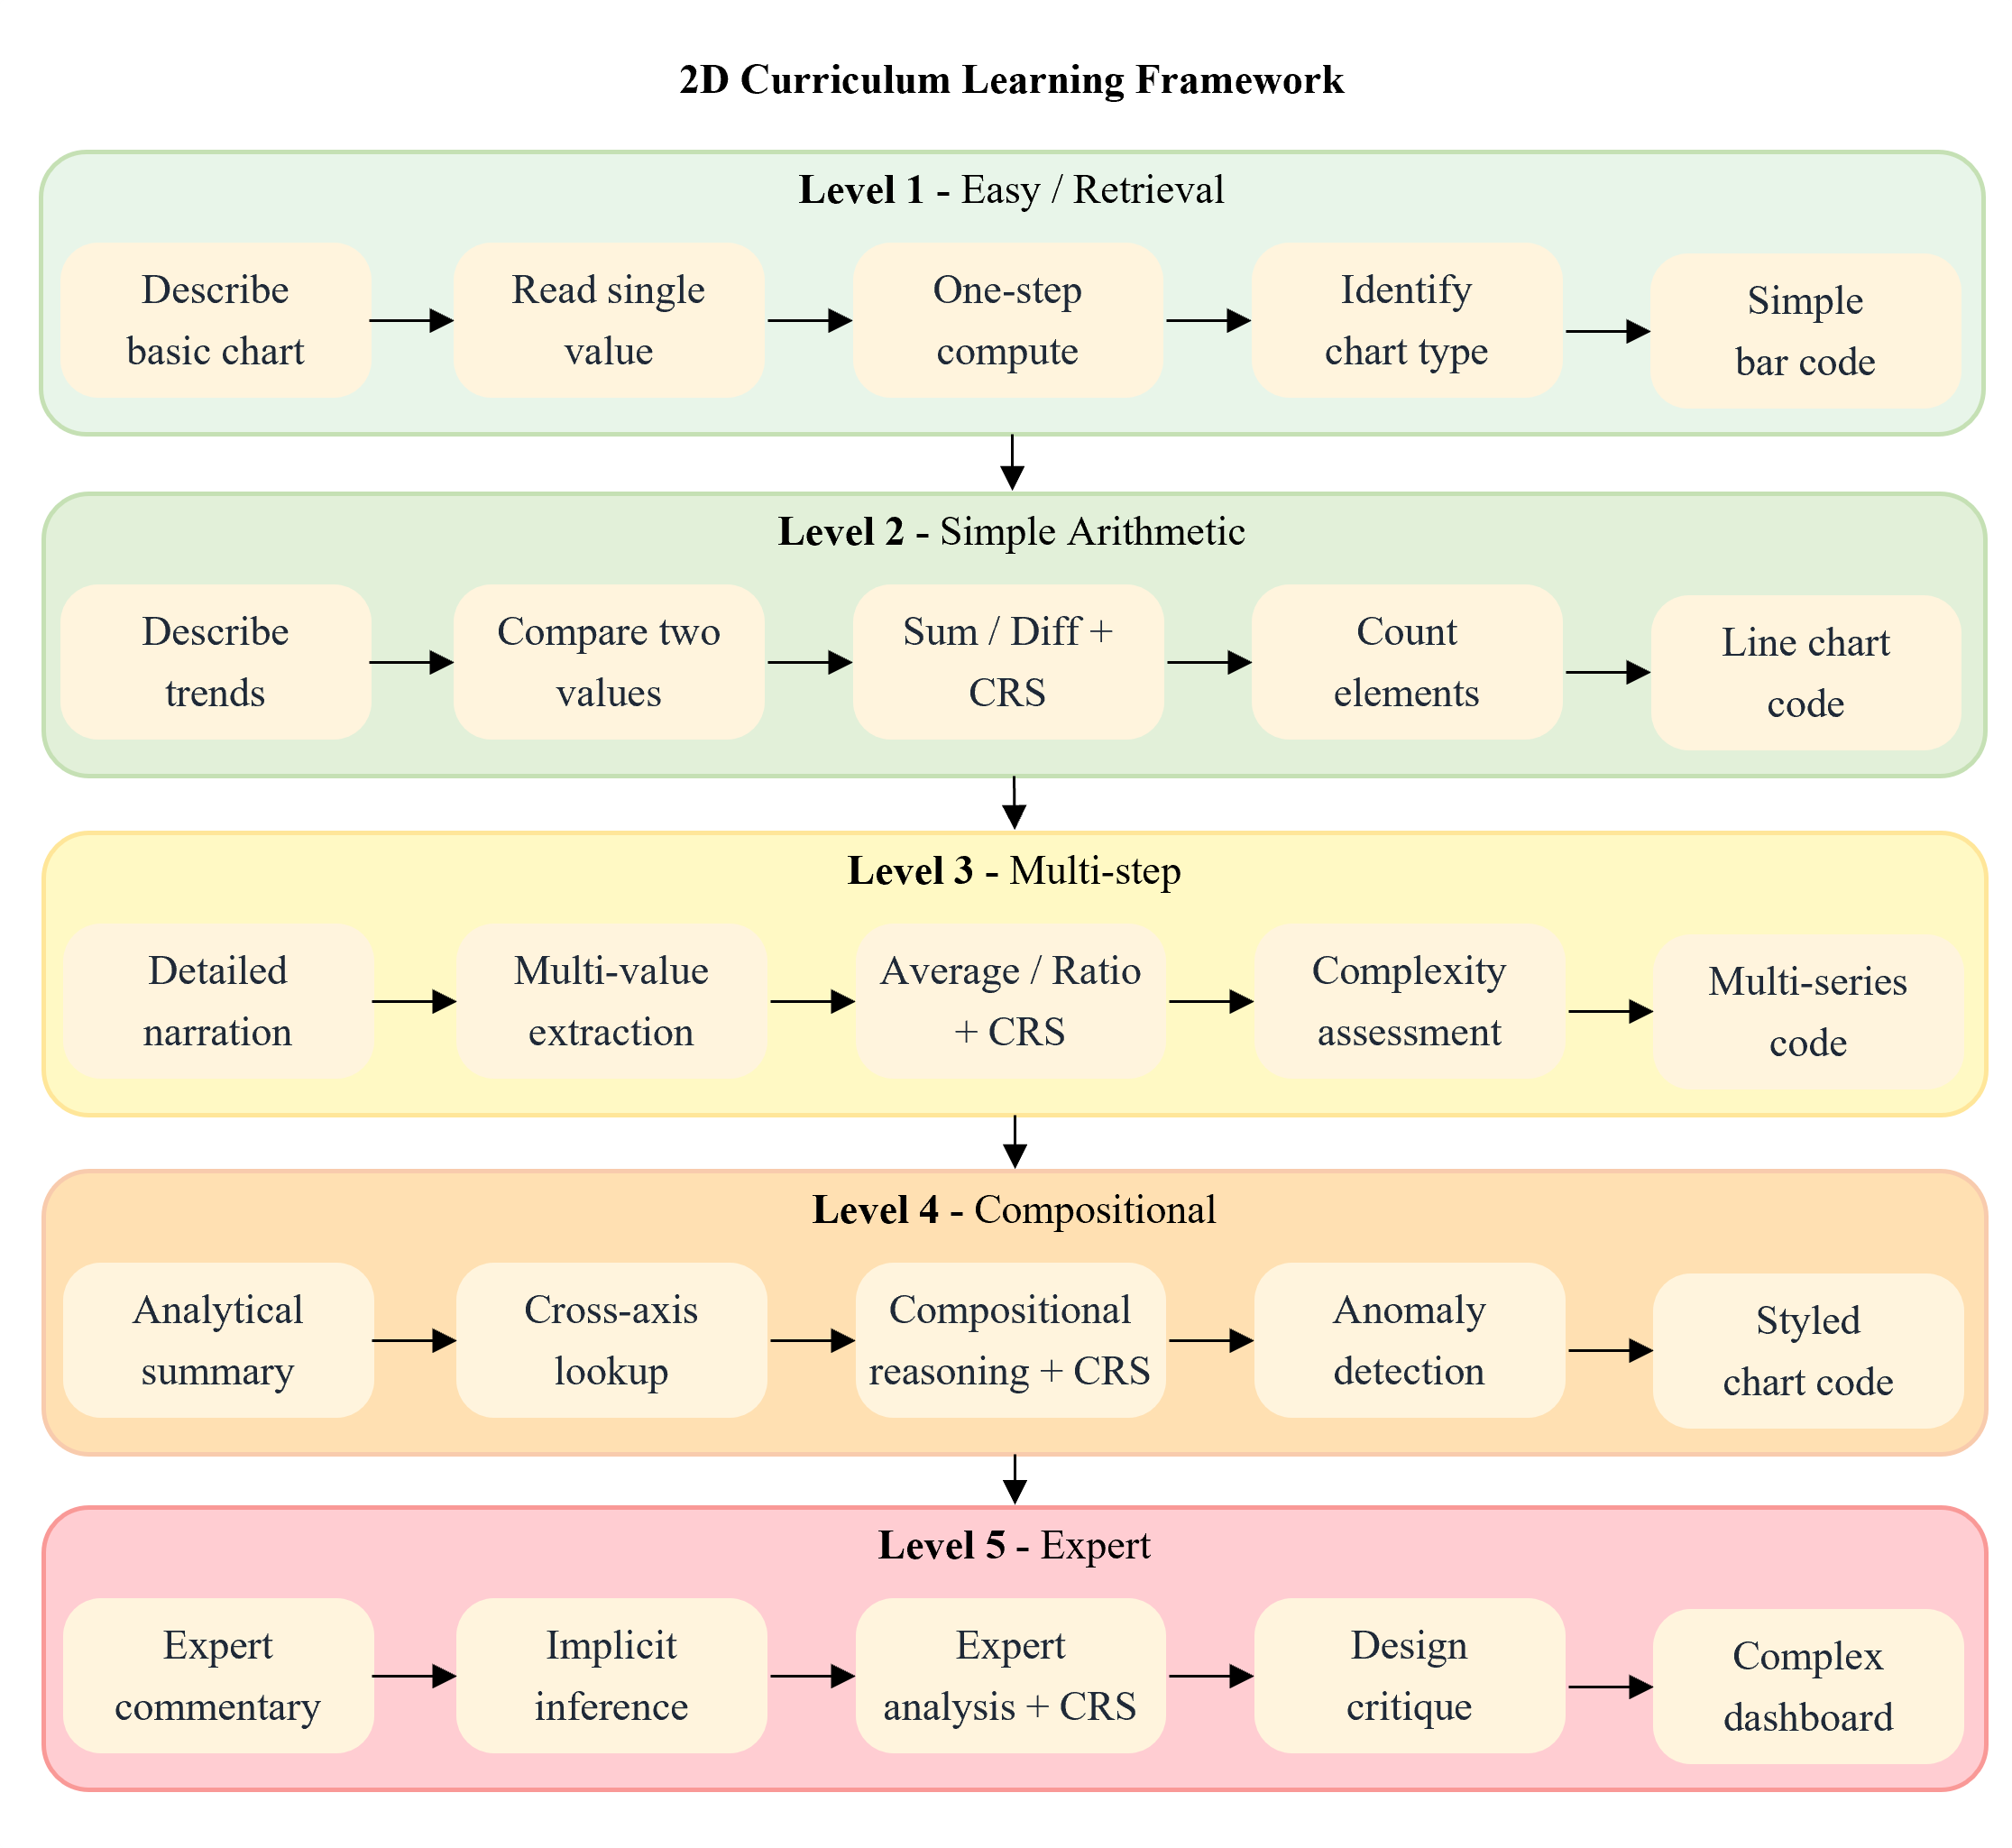
\includegraphics[width=\columnwidth]{figs/fig13_method_overview.png}
    \caption{Overview of \method{}. Training proceeds along two dimensions: horizontally through five task stages of increasing complexity, and vertically through difficulty-ordered samples within each stage. LoRA adapters are inherited across stages to preserve learned capabilities.}
    \label{fig:method_overview}
\end{figure}

We take a different approach. Drawing on the curriculum learning principle that humans learn more effectively when material is organized from simple to complex~\cite{bengio2009curriculum}, we propose \textbf{\fullmethod{} (\method{})}, a progressive fine-tuning framework that imposes structure on both \textit{what} the model learns and \textit{how} it learns (Fig.~\ref{fig:method_overview}). The horizontal dimension decomposes chart understanding into five stages of escalating task complexity: starting with basic image description to establish visual-language alignment, moving through factual question answering and multi-step reasoning, then visual element analysis, and culminating in code generation that requires synthesizing all prior skills. The vertical dimension orders training samples within each stage by difficulty, so the model encounters straightforward retrieval questions before grappling with expert-level analysis.

Two technical choices make this curriculum effective in practice. One is \textbf{Code-as-Reasoning Supervision (\crs{})}, which sidesteps the opacity of end-to-end answer prediction by training the model to produce executable Python code that makes each reasoning step explicit. When a question asks for the sum of two values, the model learns to extract those values into variables, add them, and return the result---rather than guessing a number that happens to be correct. This provides richer supervision and yields interpretable intermediate outputs. The other is \textbf{Difficulty-Aware Curriculum Data Selection (\dacds{})}, which uses a language model to score each sample's difficulty on a five-point scale. Training data is then sorted accordingly, ensuring the model masters simpler patterns before tackling harder variants.

We anchor our evaluation on ChartQA~\cite{masry2022chartqa}, the most widely adopted benchmark in this space. Using Qwen2.5-VL-7B as our base model, \method{} reaches 82.12\% accuracy---a 6.16\% absolute improvement over standard LoRA fine-tuning on the same data without curriculum structure, and competitive with models an order of magnitude larger. We achieve this using only 12K synthetic training samples, two orders of magnitude less than the pretraining corpora used by chart-specific models. This data efficiency underscores a broader point: for chart understanding, the \emph{structure} of training may matter as much as its \emph{scale}. Ablation experiments isolate the contribution of each component: adapter inheritance accounts for +4.80\%, task staging for +3.48\%, \crs{} for +2.64\%, and difficulty ordering for +1.28\%. The gains are not tied to a single model or dataset; we observe consistent improvements when applying \method{} to Qwen2.5-VL-3B and InternVL2-8B, and the trained models transfer successfully to PlotQA and FigureQA without any additional fine-tuning.

Our contributions can be summarized as follows:
\begin{itemize}
    \item A two-dimensional curriculum learning framework that jointly structures training along task complexity and sample difficulty axes, tailored for the multi-faceted nature of chart understanding.
    \item \crs{}, a supervision strategy that uses code execution traces to provide step-by-step reasoning annotations, dramatically improving performance on reasoning-intensive questions.
    \item Extensive experiments demonstrating a 6.16\% improvement over standard fine-tuning, with ablations that quantify the role of each design decision.
    \item Evidence of generalization across model architectures (Qwen-VL, InternVL) and chart understanding benchmarks (ChartQA, PlotQA, FigureQA).
\end{itemize}

\section{Related Work}
\paragraph{Chart Understanding.}
The earliest systems for chart question answering adopted a two-stage pipeline: detect and parse visual elements into a structured table, then apply standard reasoning techniques to the extracted data~\cite{kafle2018dvqa,kahou2017figureqa}. While conceptually clean, this decomposition introduces error propagation---mistakes in parsing compound through downstream reasoning. More recent work has gravitated toward end-to-end architectures that sidestep explicit table extraction. Pix2Struct~\cite{lee2023pix2struct} pretrains on web screenshots to learn general document layout understanding, which transfers surprisingly well to charts. MatCha~\cite{liu2023matcha} augments this foundation with mathematical reasoning pretraining, while UniChart~\cite{masry2023unichart} designs chart-specific auxiliary tasks such as chart-to-table conversion. DePlot~\cite{liu2023deplot} takes a hybrid approach, training a chart-to-table module and delegating reasoning to a separate large language model. ChartLlama~\cite{han2023chartllama} instruction-tunes a vision-language model directly on chart data. These specialized systems have pushed accuracy upward, but typically require large amounts of chart-specific pretraining data---a resource constraint that limits their accessibility. Our work explores whether careful training curriculum design can achieve comparable results with far less data, adapting general-purpose VLMs using only around 12K samples.

\paragraph{Vision-Language Models.}
The past two years have seen rapid progress in vision-language models capable of general visual understanding~\cite{liu2024visual,chen2024internvl,bai2023qwen}. Proprietary systems like GPT-4V~\cite{openai2023gpt4v} and Claude 3.5~\cite{anthropic2024claude} demonstrate impressive zero-shot chart comprehension, though their closed nature precludes fine-tuning for specialized tasks. On the open-source side, LLaVA~\cite{liu2024visual}, Qwen-VL~\cite{bai2023qwen}, and InternVL~\cite{chen2024internvl} offer strong starting points for domain adaptation. These models already possess considerable visual and linguistic capabilities; the question is how best to steer them toward chart understanding without requiring massive retraining. Our experiments suggest that the answer lies less in the quantity of data and more in how training is organized.

\paragraph{Curriculum Learning.}
The idea of presenting training examples in a meaningful order---easy before hard, simple before complex---dates back at least to~\cite{bengio2009curriculum}, who showed that such curricula can accelerate convergence and improve generalization. Since then, curriculum learning has been applied across machine learning, from image classification~\cite{hacohen2019power} to natural language understanding~\cite{xu2020curriculum}. A comprehensive survey by~\cite{soviany2022curriculum} catalogs these applications and identifies open challenges. Vision-language settings have received less attention, with existing work largely focused on single-dimension difficulty orderings~\cite{shen2021much}. We extend this paradigm to two dimensions---task complexity and sample difficulty---showing that the combination yields larger gains than either dimension alone.

\paragraph{Reasoning in Vision-Language Models.}
Endowing VLMs with multi-step reasoning capabilities remains an open problem. Chain-of-thought prompting~\cite{wei2022chain} can elicit reasoning at inference time, but provides no training signal. Program-aided approaches~\cite{gao2023pal,chen2022program} generate code as an intermediate reasoning artifact, making computation explicit and verifiable. Recent efforts have sought to incorporate reasoning chains during training, either through synthetic data generation~\cite{lu2024mathvista} or knowledge distillation from larger models~\cite{shao2024visual}. Our \crs{} method draws on the insight that code is a natural medium for expressing computation, but differs from PAL and PoT in a fundamental way. PAL and PoT are \emph{inference-time} mechanisms: the model generates code at test time, which is then executed externally to obtain the answer. \crs{}, by contrast, is a \emph{training-time} supervision strategy. During training, executable Python code traces serve as structured annotations that teach the model to reason step by step---extracting values, performing arithmetic, and returning answers, each step grounded in the chart's visual content. At inference, the model produces direct text answers without any external code execution; the reasoning patterns learned through \crs{} are internalized into the model weights and transferred to downstream QA tasks via adapter inheritance (\S\ref{sec:adapter}). This means \crs{}-trained models carry no runtime dependency on a Python interpreter, and the benefits of code-based supervision persist even when the model is evaluated in a standard QA format.

\section{Method}
This section describes \fullmethod{} (\method{}), our progressive fine-tuning framework for chart understanding. The core idea is to impose structure on the training process along two complementary dimensions---task complexity and sample difficulty---rather than treating all training data as interchangeable. Fig.~\ref{fig:method_overview} provides an overview.

\subsection{Problem Formulation}
\label{sec:problem}
Given a chart image $I$ and a natural language question $q$, the task is to produce an answer $a$ that correctly addresses the question in light of the visual content. This deceptively simple formulation masks considerable underlying complexity. Chart understanding is not a single capability but a bundle of interrelated skills: the model must recognize visual elements (bars, lines, axes, legends), map textual labels to their visual referents, extract numerical values from positions or annotations, perform arithmetic when the question calls for it, and reason about relationships that span multiple data points. Training a model to acquire all of these skills at once, with no guidance about order or difficulty, places a substantial burden on the learning algorithm.

Our approach decomposes this burden by organizing training into a sequence of progressively complex tasks, each of which builds on capabilities established in earlier stages.

\subsection{Two-Dimensional Curriculum Design}
\label{sec:2d_curriculum}
\paragraph{Horizontal Dimension: Task Complexity.}
We structure training into five stages, each targeting a distinct facet of chart understanding:
\begin{enumerate}
    \item \textbf{Stage 1: Image Description.} The model learns to produce detailed textual descriptions of chart contents---what type of chart it is, what the axes represent, what trends are visible. This stage establishes a foundation of visual-language alignment before any question answering is attempted.
    \item \textbf{Stage 2: Basic VQA.} Here the model begins answering factual questions: direct value lookups (``What is the sales figure for March?'') and simple comparisons (``Which month had higher revenue?''). These require accurate value extraction but minimal reasoning.
    \item \textbf{Stage 3: Reasoning VQA.} Questions now demand multi-step reasoning---computing averages, identifying trends, combining information from different parts of the chart. We supervise this stage using \crs{} (described in \S\ref{sec:crs}), which provides explicit step-by-step guidance.
    \item \textbf{Stage 4: Visual Analysis.} The model performs fine-grained visual inspection: counting elements, classifying chart types, assessing visual complexity. This stage reinforces detailed visual understanding that complements the reasoning skills acquired earlier.
    \item \textbf{Stage 5: Code Generation.} The final stage asks the model to generate executable Python code that would reproduce the chart from data. This is the most demanding task, requiring synthesis of visual structure, data values, and programming knowledge.
\end{enumerate}
The ordering reflects a deliberate pedagogical logic. Basic description and value extraction lay the groundwork for reasoning; visual analysis reinforces perceptual precision; code generation integrates everything. Each stage inherits knowledge from the previous one (as detailed in \S\ref{sec:adapter}), so the model never starts from scratch.

\paragraph{Vertical Dimension: Sample Difficulty.}
Even within a single task stage, not all samples are equally challenging. We therefore impose a second level of curriculum by ordering training samples from easy to hard within each stage. Difficulty is assessed on a five-point scale:
\begin{itemize}
    \item \textbf{Level 1:} Direct retrieval---the answer can be read off the chart with no computation.
    \item \textbf{Level 2:} One-step arithmetic---a single operation on directly extracted values.
    \item \textbf{Level 3:} Multi-step reasoning---three to five chained operations.
    \item \textbf{Level 4:} Compositional questions---combining multiple reasoning patterns.
    \item \textbf{Level 5:} Expert-level analysis---questions that require domain knowledge or nuanced interpretation.
\end{itemize}
This vertical ordering ensures that within each task stage, the model masters simpler variants before confronting harder ones.

\subsection{Code-as-Reasoning Supervision}
\label{sec:crs}
A recurring obstacle in teaching VLMs to reason is the opacity of the learning signal. Standard training provides (question, answer) pairs with nothing in between---the model sees the destination but not the path. This is especially problematic for multi-step reasoning, where a correct answer might be reached through any number of computational routes, some robust and others fragile.

We address this with \textbf{Code-as-Reasoning Supervision (\crs{})}, which makes reasoning explicit by training the model to generate executable Python code rather than direct answers. For a question like ``What is the sum of Q1 and Q2?'', the expected output might look like:
\begin{small}
\begin{verbatim}
# Extract values from chart
values = {'Q1': 77, 'Q2': 18, 'Q3': 45, 'Q4': 62}
# Retrieve the relevant entries
q1_val = values['Q1']  # 77
q2_val = values['Q2']  # 18
# Compute the answer
answer = q1_val + q2_val  # 95
\end{verbatim}
\end{small}
Each line serves as a supervision signal: the model learns not only what the answer is but how to arrive at it through a sequence of grounded operations. The code is executable, so its correctness can be verified programmatically. And the structured format leaves little room for shortcuts---the model cannot simply guess a plausible number without first going through the extraction and computation steps.

\paragraph{Inference with \crs{}.}
An important distinction concerns how \crs{}-trained models operate at inference time. During evaluation on standard benchmarks like ChartQA, we do \emph{not} execute the generated code externally. Instead, the model uses the Stage 2 or Stage 4 adapter, which produces direct text answers in the format expected by the benchmark. The \crs{}-trained Stage 3 adapter serves a different purpose: it internalizes step-by-step reasoning patterns during training, and this structured reasoning capability transfers to the QA adapters through adapter inheritance. When deployed in reasoning-heavy scenarios, the Stage 3 adapter can generate code traces for interpretability, but standard QA evaluation relies on text-based answer generation. This design means that performance gains on ChartQA stem from improved reasoning internalization, not from external code execution.

\subsection{Difficulty-Aware Data Selection}
\label{sec:dacds}
To implement the vertical curriculum, we need a reliable way to assess sample difficulty. Manual annotation at scale is impractical, so we leverage \textbf{Qwen2.5-72B-Instruct} as an automated difficulty scorer. Given a question-answer pair and the chart context, the model is prompted to assign a difficulty level from 1 to 5 based on the number of reasoning steps required, the complexity of the arithmetic involved, and whether domain-specific knowledge is needed. Training data within each stage is then sorted by this score in ascending order.

This \textbf{Difficulty-Aware Curriculum Data Selection (\dacds{})} strategy complements the horizontal task curriculum. The horizontal dimension determines \textit{what} capability to train next; the vertical dimension determines \textit{how} to train it most efficiently. Together, they guide the model through a two-dimensional progression from simple and easy to complex and hard.

\subsection{Progressive Fine-Tuning with Adapter Inheritance}
\label{sec:adapter}
We realize the curriculum using LoRA adapters~\cite{hu2022lora} with a crucial twist: adapters are inherited across stages. Formally, let $\theta_0$ denote the pretrained VLM parameters and $\Delta\theta_s$ denote the LoRA adapter weights at stage $s$. The training procedure is:
\begin{align}
    \Delta\theta_1 &= \text{Train}(\theta_0, \mathcal{D}_1) \label{eq:stage1} \\
    \Delta\theta_s &= \text{Train}(\theta_0 + \Delta\theta_{s-1}, \mathcal{D}_s), \quad s = 2, \ldots, 5 \label{eq:stages}
\end{align}
where $\mathcal{D}_s$ is the difficulty-sorted training data for stage $s$. The key insight is in Eq.~\ref{eq:stages}: each stage initializes from the \emph{previous} stage's adapter rather than from the pretrained model. This enables cumulative knowledge building---Stage 2 inherits the visual-language alignment from Stage 1, Stage 3 inherits the QA patterns from Stage 2, and so on.

This inheritance mechanism creates a family of specialized adapters---one per stage---that can be deployed independently at inference time. For general question answering, the Stage 2 or Stage 4 adapter is often best. For complex reasoning, Stage 3 excels. For code generation, Stage 5 is the natural choice. Users can switch adapters depending on the task at hand, trading off generality for specialization.

\begin{figure}[!t]
    \centering
    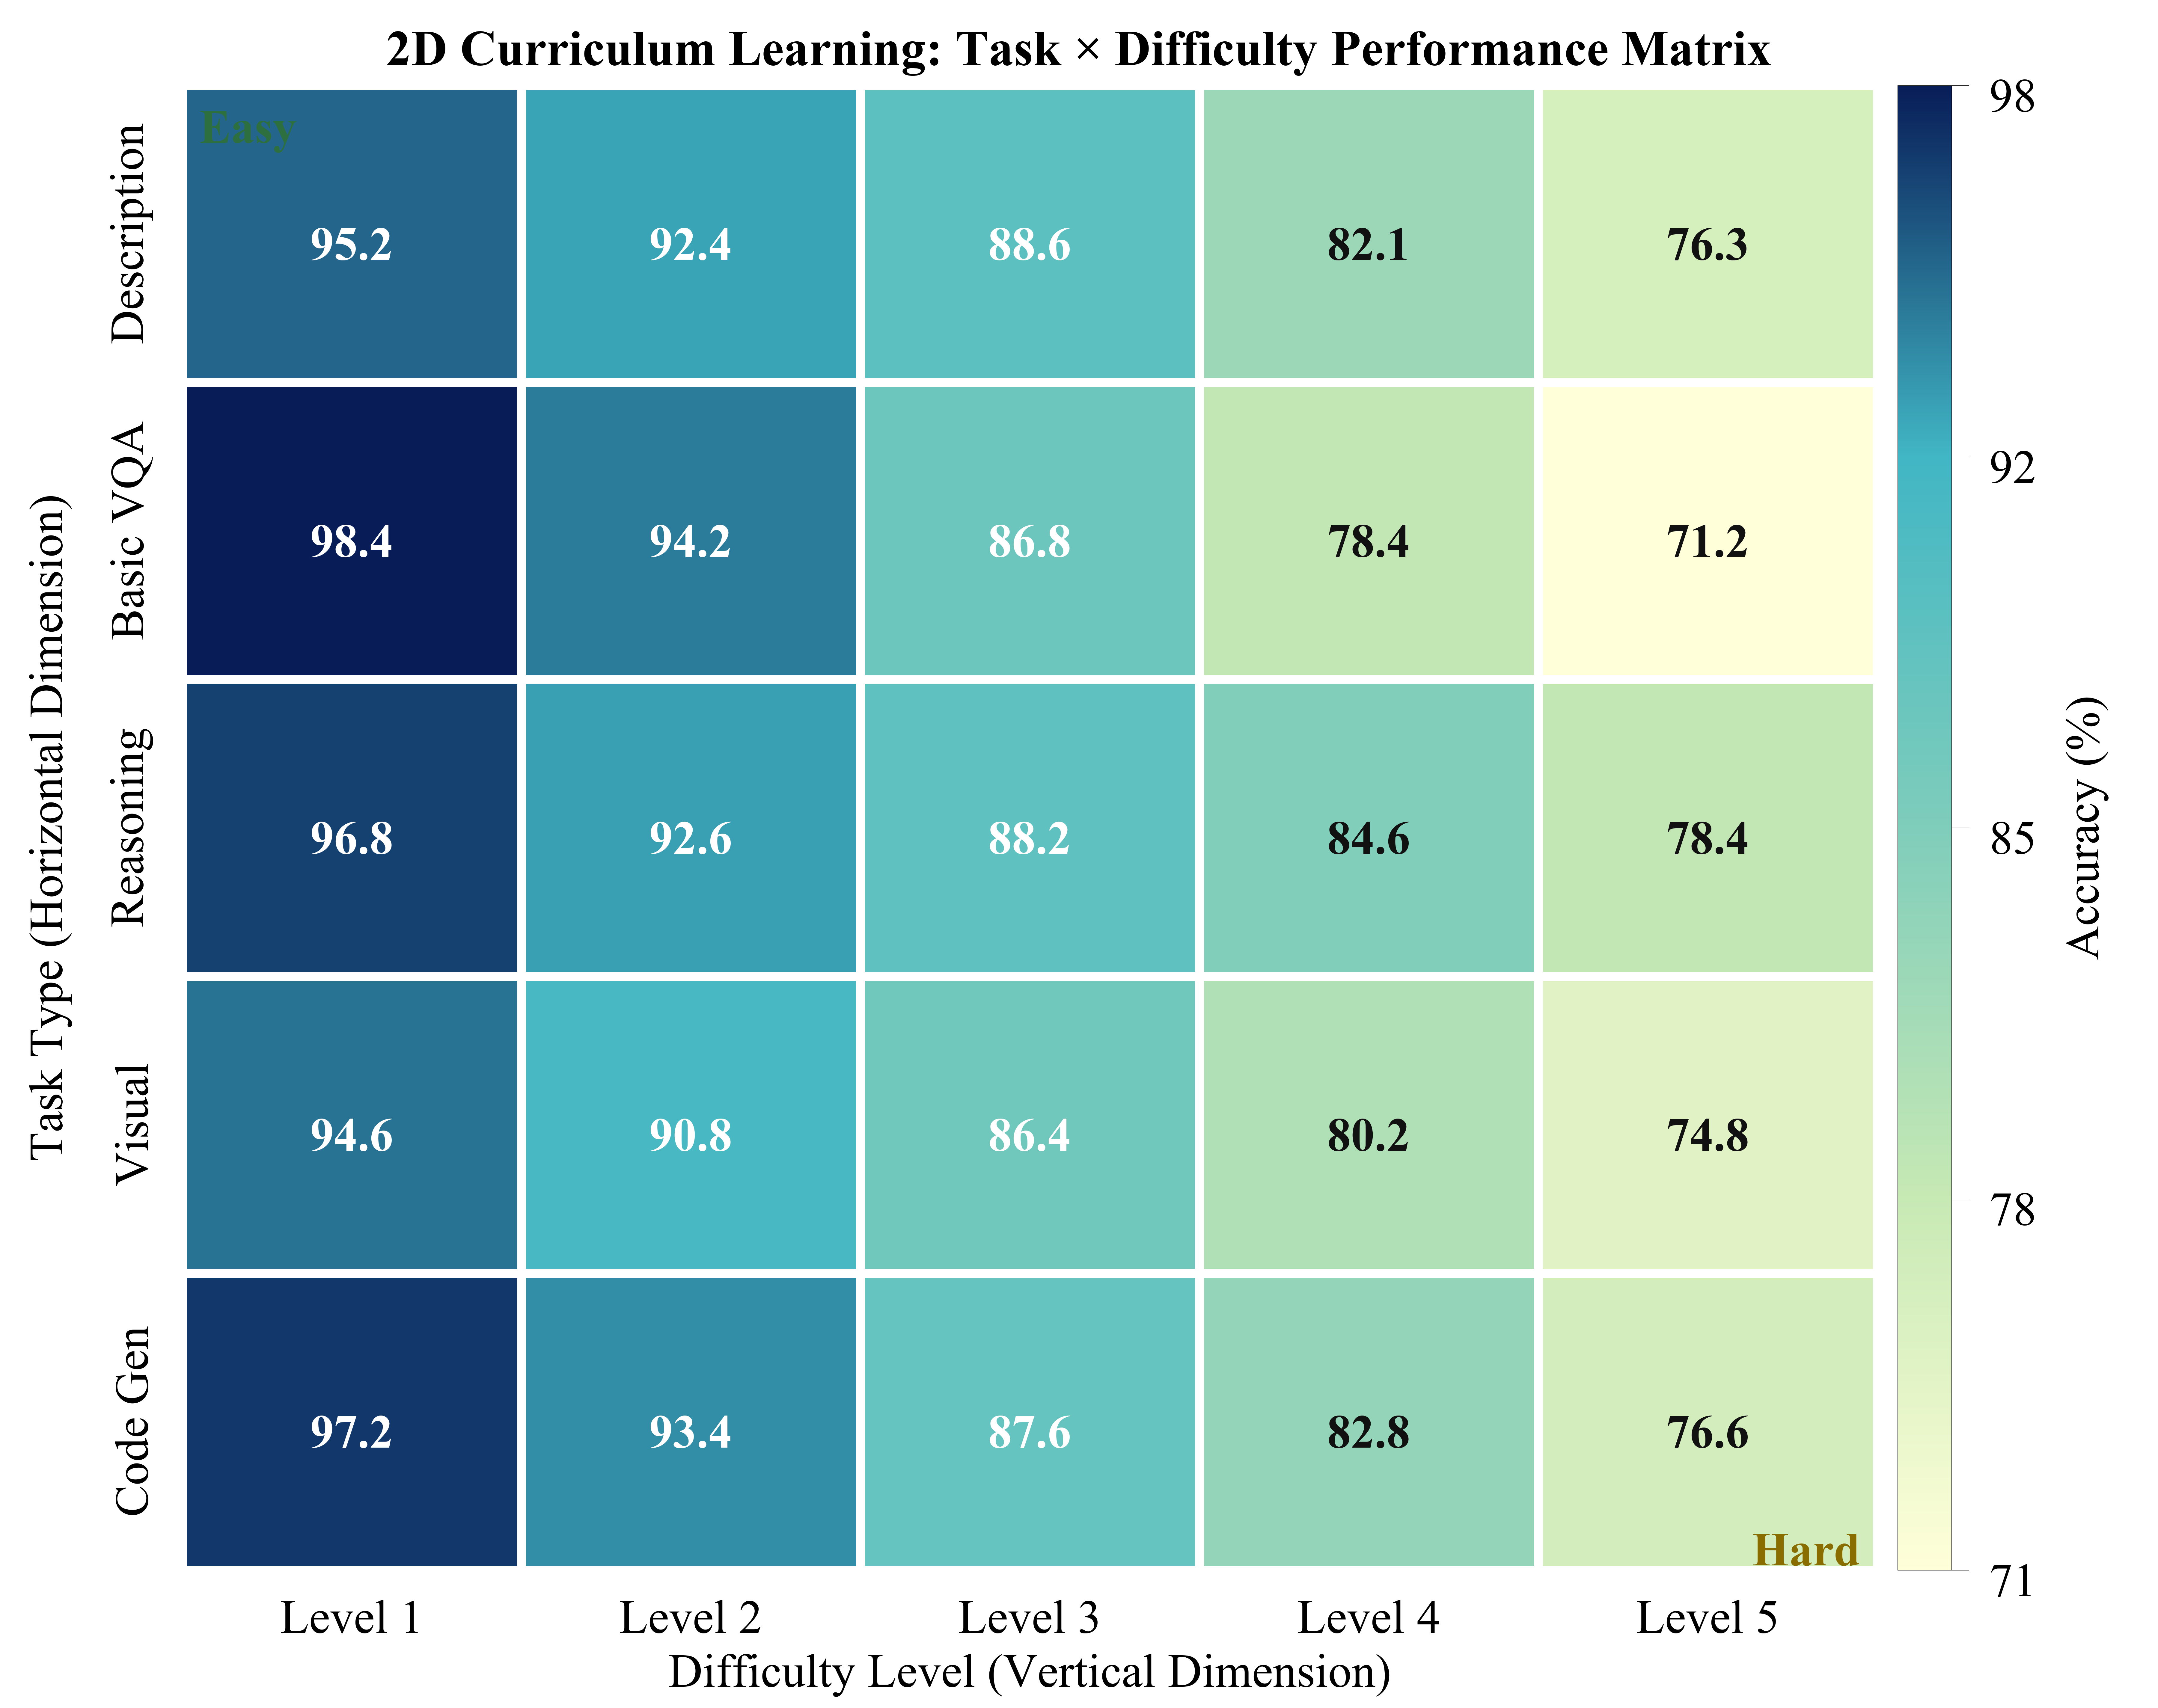
\includegraphics[width=\columnwidth]{figs/fig9_2d_curriculum_heatmap.png}
    \caption{Performance heatmap across task types (rows) and difficulty levels (columns). Performance is highest in the top-left (simple tasks, easy samples) and lowest in the bottom-right (complex tasks, hard samples), reflecting the structure of the 2D curriculum.}
    \label{fig:heatmap}
\end{figure}

Fig.~\ref{fig:heatmap} visualizes the resulting performance landscape. As expected, accuracy is highest for simpler tasks at lower difficulty levels and decreases as we move toward complex tasks and harder samples. The diagonal gradient confirms that our two-dimensional curriculum captures a meaningful learning trajectory.

\section{Experiments}
\subsection{Experimental Setup}
\label{sec:setup}
\paragraph{Training Data.}
We generate a synthetic dataset of 1,973 chart images using Python matplotlib, with data distributions, axis configurations, color schemes, and visual styles randomized across 10 scenarios (business, science, economics, healthcare, and others) and 5 chart types (bar, line, pie, scatter, area). For each chart, question-answer pairs are generated by Qwen2.5-72B-Instruct, which receives the underlying data table and chart metadata as context. Reasoning chain annotations (used for \crs{} in Stage 3) are produced by the same model and validated programmatically: generated Python code is executed to verify that it produces the expected numerical answer, and samples with execution errors are filtered. From these images, we derive training samples across our five task stages: 1,775 samples each for image description, basic VQA, reasoning VQA, and code generation, plus 5,327 samples for visual analysis (which includes three subtasks per image). The complete training set totals 12,427 samples---a deliberately modest amount, as one of our goals is to test whether curriculum structure can compensate for data scale. Each sample is annotated with a difficulty level (1--5) assessed by Qwen2.5-72B-Instruct on a scale based on the number of reasoning steps, arithmetic complexity, and domain knowledge required.

\paragraph{Base Models.}
Our primary experiments use Qwen2.5-VL-7B-Instruct~\cite{bai2023qwen}. To assess generalization, we additionally train and evaluate on Qwen2.5-VL-3B-Instruct and InternVL2-8B~\cite{chen2024internvl}, which differ in both scale and architecture.

\paragraph{Training Configuration.}
We adopt LoRA~\cite{hu2022lora} with rank 8 and scaling factor $\alpha=16$. Each stage trains for 10 epochs with an effective batch size of 16. Learning rates taper across stages: $1\times10^{-4}$ for Stage 1, $5\times10^{-5}$ for Stage 2, $3\times10^{-5}$ for Stages 3 and 4, and $2\times10^{-5}$ for Stage 5. All experiments are conducted on a single NVIDIA RTX 5090 GPU; full \method{} training requires approximately 21 hours. Complete hyperparameters are provided in the supplementary material.

\paragraph{Evaluation Benchmarks.}
The primary benchmark is ChartQA~\cite{masry2022chartqa}, which contains 9.6K human-annotated and 23.1K machine-generated question-answer pairs over real-world charts. We report accuracy on the official test split (2,500 samples). For cross-dataset evaluation, we use PlotQA~\cite{methani2020plotqa} (scientific plots with reasoning-intensive questions) and FigureQA~\cite{kahou2017figureqa} (synthetic charts with binary yes/no questions) in a zero-shot setting---models trained only on our synthetic data are evaluated directly without any fine-tuning on the target datasets.

\subsection{Main Results}
\label{sec:main_results}
\begin{table}[!t]
\centering
\small
\begin{tabular}{lccc}
\toprule
\textbf{Method} & \textbf{Params} & \textbf{Train Data} & \textbf{Acc.} \\
\midrule
\multicolumn{4}{l}{\textit{Proprietary Models}} \\
Claude 3.5 Sonnet & --- & --- & 90.8 \\
GPT-4V & --- & --- & 85.7 \\
\midrule
\multicolumn{4}{l}{\textit{Open-Source VLMs (zero-shot)}} \\
Qwen2.5-VL-72B & 72B & --- & 89.5 \\
InternVL2-Pro & 40B & --- & 83.8 \\
LLaVA-1.6-34B & 34B & --- & 68.3 \\
\midrule
\multicolumn{4}{l}{\textit{Chart-Specific Models}} \\
ChartLlama & 13B & 160K & 69.4 \\
MatCha & 282M & $\sim$2M & 64.2 \\
UniChart & 140M & 611K & 60.8 \\
Pix2Struct & 282M & 80M & 56.0 \\
DePlot & 282M & $\sim$2M & 54.3 \\
\midrule
Qwen2.5-VL-7B & 7B & --- & 80.28 \\
\textbf{Ours (\method{})} & \textbf{7B} & \textbf{12K} & \textbf{82.12} \\
\bottomrule
\end{tabular}
\caption{Comparison with existing methods on ChartQA. ``Train Data'' indicates the volume of chart-specific training data used. Our method achieves 82.12\% accuracy using only 12K synthetic samples---orders of magnitude less than chart-specific models.}
\label{tab:sota}
\end{table}

Table~\ref{tab:sota} reveals two patterns. First, \method{} is remarkably data-efficient: with only 12K synthetic samples, it outperforms models trained on 50--150$\times$ more chart-specific data. We note that chart-specific models (MatCha, UniChart, Pix2Struct) use substantially smaller backbones (140M--282M parameters), so the comparison primarily illustrates data efficiency rather than architectural superiority. Second, at the 7B scale, \method{} closes the gap to much larger models: it trails InternVL2-Pro (40B) by only 1.7 points and Qwen2.5-VL-72B by 7.4 points, despite being 5--10$\times$ smaller.

Relative to the Qwen2.5-VL-7B zero-shot baseline (80.28\%), \method{} adds 1.84 absolute points. The zero-shot baseline is already strong---Qwen2.5-VL-7B is a capable general-purpose VLM---yet our curriculum still finds room for improvement, particularly on questions requiring multi-step reasoning. The more informative comparison is against standard LoRA fine-tuning on the same 12K samples without any curriculum structure (75.96\%), over which \method{} achieves a 6.16\% improvement. This gap isolates the contribution of curriculum design from model capability and data volume.

\subsection{Ablation Study}
\label{sec:ablation}
\begin{table}[!t]
\centering
\small
\begin{tabular}{lccccc}
\toprule
\textbf{Configuration} & \textbf{Stage} & \textbf{Diff.} & \textbf{CRS} & \textbf{Inh.} & \textbf{Acc.} \\
\midrule
Full \method{} & \checkmark & \checkmark & \checkmark & \checkmark & 82.12 \\
\midrule
w/o Staging & --- & \checkmark & \checkmark & --- & 78.64 \\
w/o Difficulty & \checkmark & --- & \checkmark & \checkmark & 80.84 \\
w/o CRS & \checkmark & \checkmark & --- & \checkmark & 79.48 \\
w/o Inheritance & \checkmark & \checkmark & \checkmark & --- & 77.32 \\
\midrule
Standard LoRA SFT & --- & --- & --- & --- & 75.96 \\
\bottomrule
\end{tabular}
\caption{Ablation study on ChartQA. ``Standard LoRA SFT'' trains on the same 12K samples with all tasks and difficulty levels mixed together, without any curriculum structure. Removing any component hurts performance; adapter inheritance (Inh.) and task staging contribute the most.}
\label{tab:ablation}
\end{table}

To understand which components of \method{} contribute most, we run an ablation study (Table~\ref{tab:ablation}). Each row removes or disables one design element while keeping others intact.

\textbf{Adapter inheritance} turns out to be the single most important factor. When we train each stage from the pretrained model rather than inheriting from the previous stage, accuracy drops to 77.32\%---a 4.80\% loss. This makes sense: without inheritance, the model must rediscover foundational capabilities at each stage rather than building on what came before. The curriculum's progressive structure is wasted if knowledge does not flow forward.

\textbf{Task staging} contributes 3.48\%. Mixing all training data together removes the horizontal curriculum, and accuracy falls to 78.64\%. Interestingly, this configuration still includes difficulty ordering, but without the task decomposition, the benefit is diminished.

\textbf{Code-as-Reasoning Supervision} accounts for 2.64\%. Disabling \crs{} in Stage 3 hurts reasoning-intensive questions disproportionately. On our internal reasoning benchmark, accuracy drops from 100\% to 72.4\% when \crs{} is removed, consistent with the intuition that explicit reasoning supervision is especially valuable for multi-step computation.

\textbf{Difficulty ordering} provides a smaller but reliable 1.28\% gain. Shuffling samples within each stage reduces accuracy to 80.84\%. While less dramatic than the other components, this confirms that even within a fixed task, easier-first ordering helps.

Taken together, the full \method{} configuration outperforms standard LoRA SFT by 6.16\%. The components are not redundant: each addresses a different aspect of the learning problem, and their benefits accumulate.

\paragraph{Comparison with 1D Curriculum Learning.}
Our ablation configurations naturally correspond to one-dimensional curriculum baselines. Removing difficulty ordering (w/o Difficulty, 80.84\%) is equivalent to a \emph{task-only} curriculum that stages training across five tasks but presents samples in random order within each stage. Removing task staging (w/o Staging, 78.64\%) corresponds to a \emph{difficulty-only} curriculum that orders all samples by difficulty but makes no distinction between task types. The progression is clear: 2D-CL (82.12\%) $>$ 1D-Task (80.84\%) $>$ 1D-Difficulty (78.64\%) $>$ No curriculum (75.96\%). Task decomposition provides greater benefit than difficulty ordering alone, but combining both dimensions yields the best result.

\subsection{Generalization Experiments}
\label{sec:generalization}
\begin{figure*}[!t]
    \centering
    \subfloat[Ablation study]{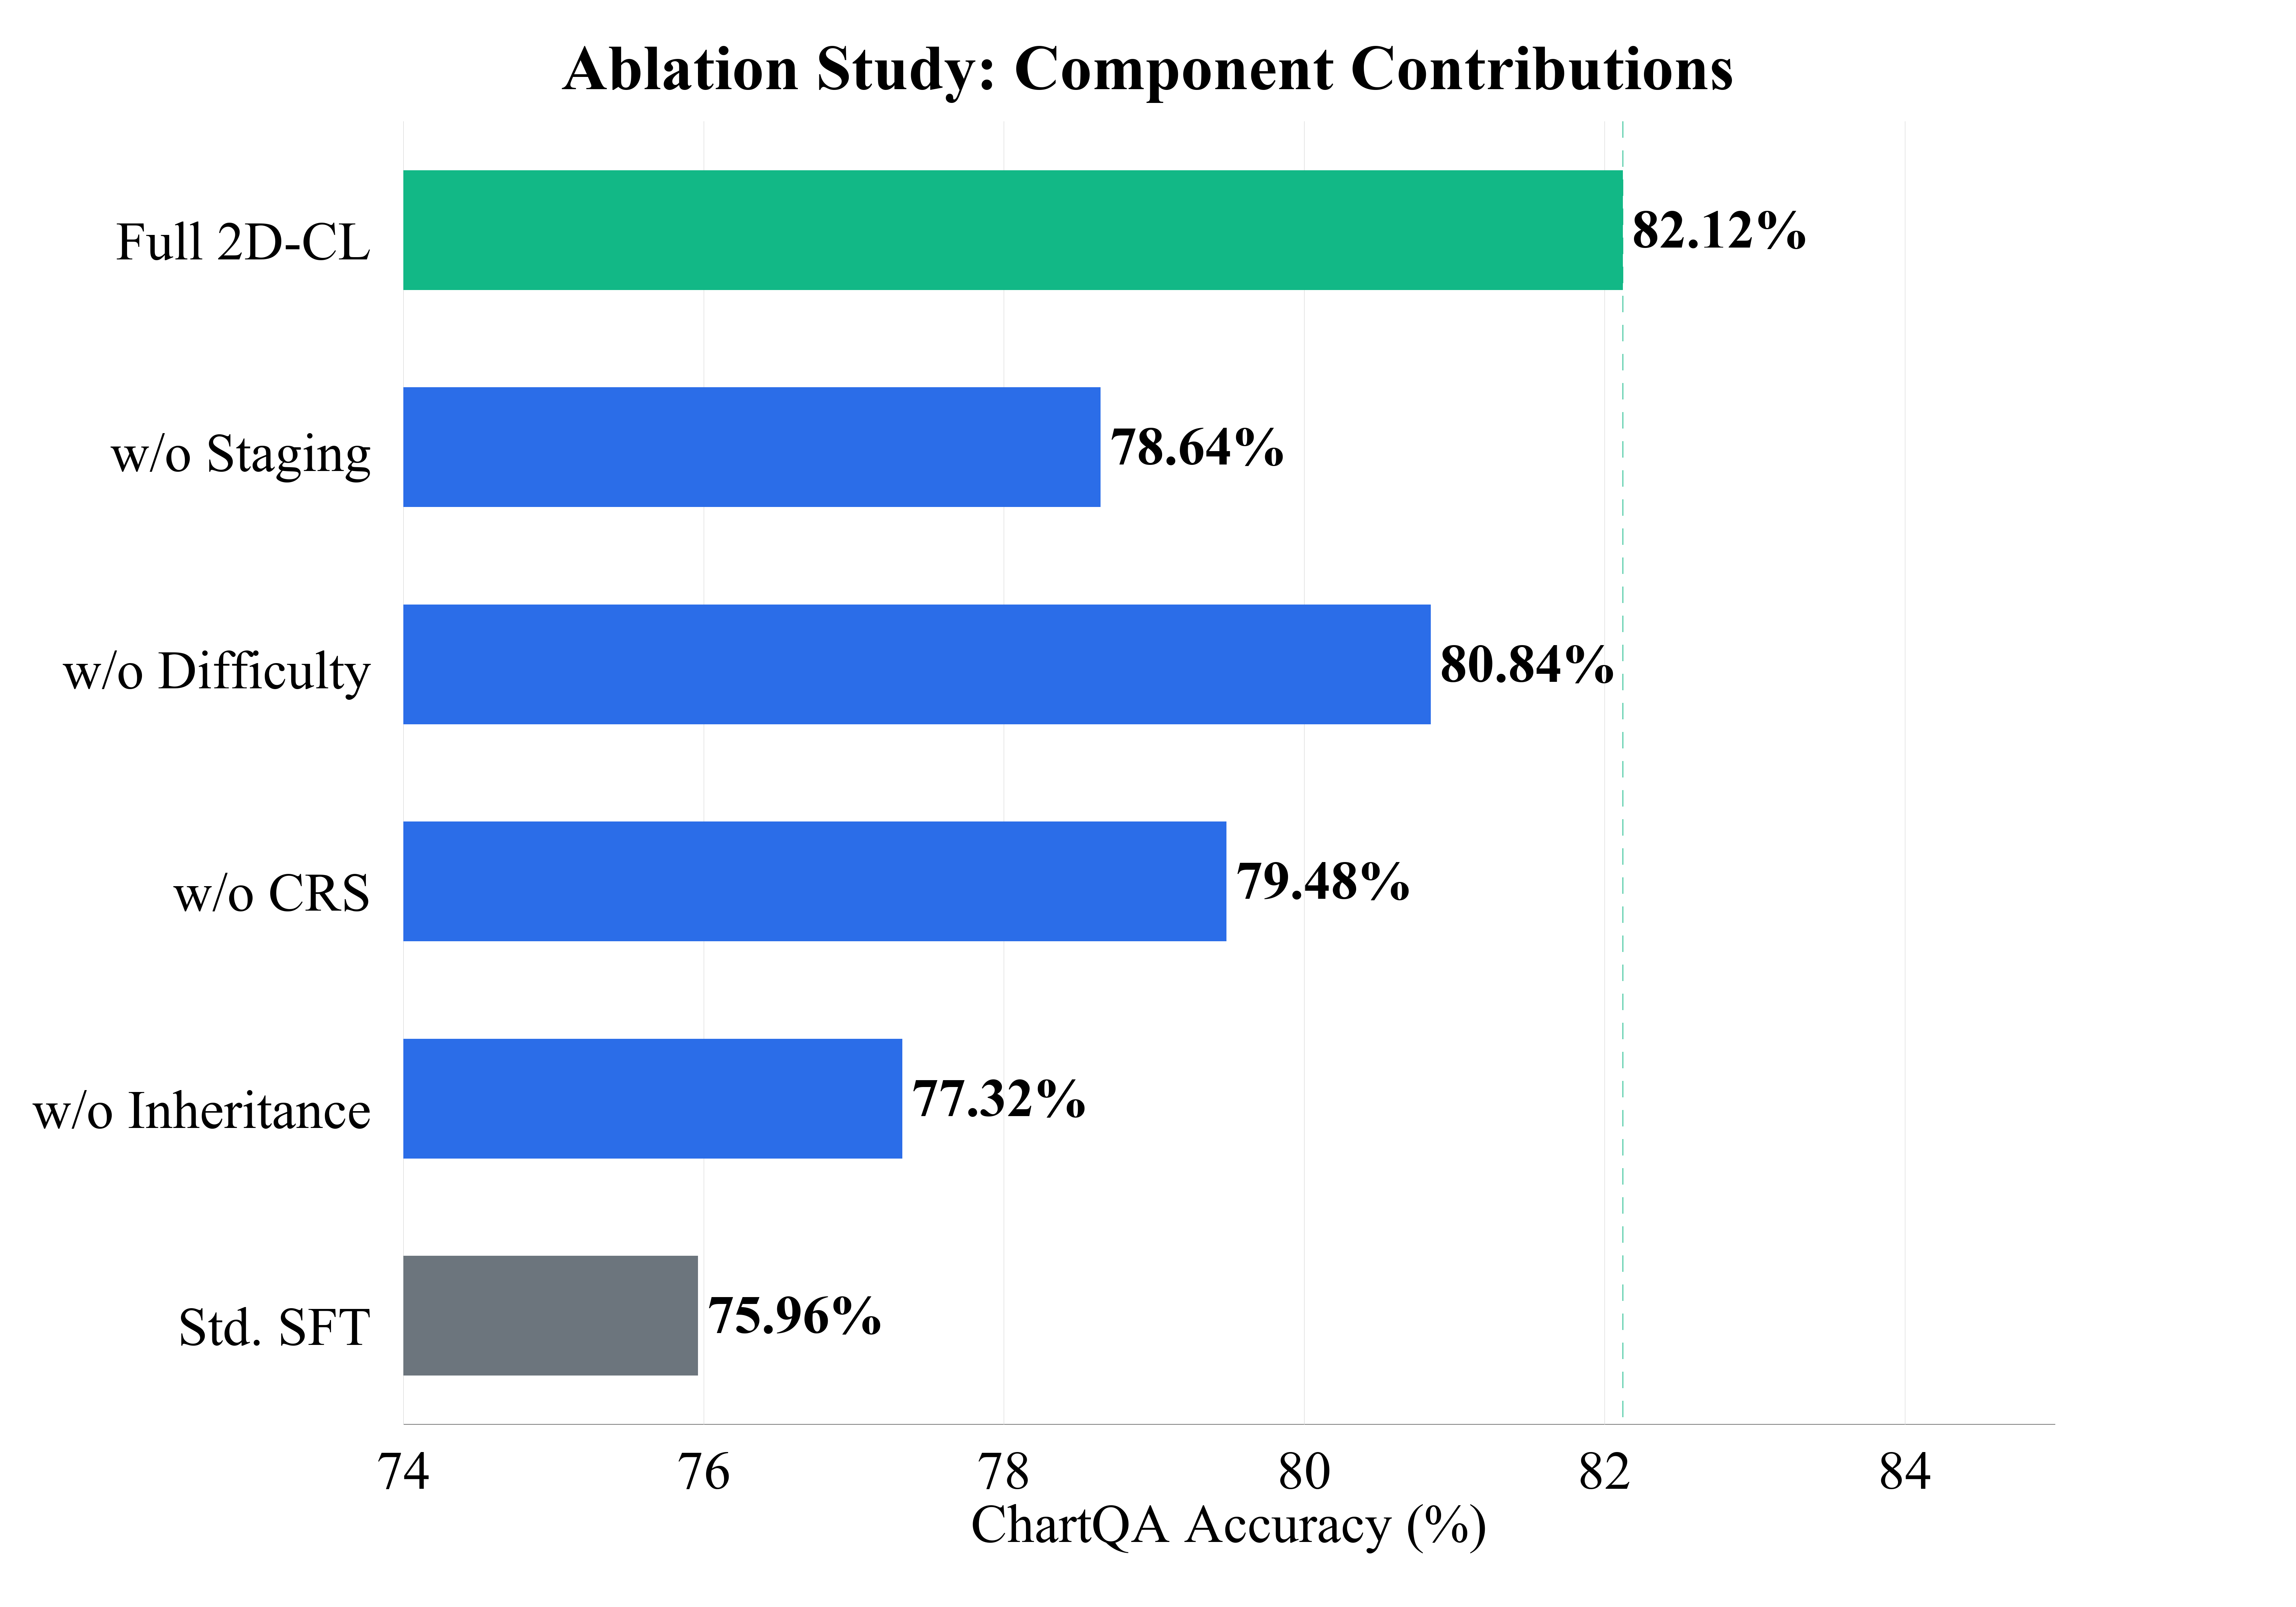
\includegraphics[width=0.32\textwidth]{figs/fig3_ablation_study.png}\label{fig:exp_ablation}}
    \hfil
    \subfloat[Cross-model generalization]{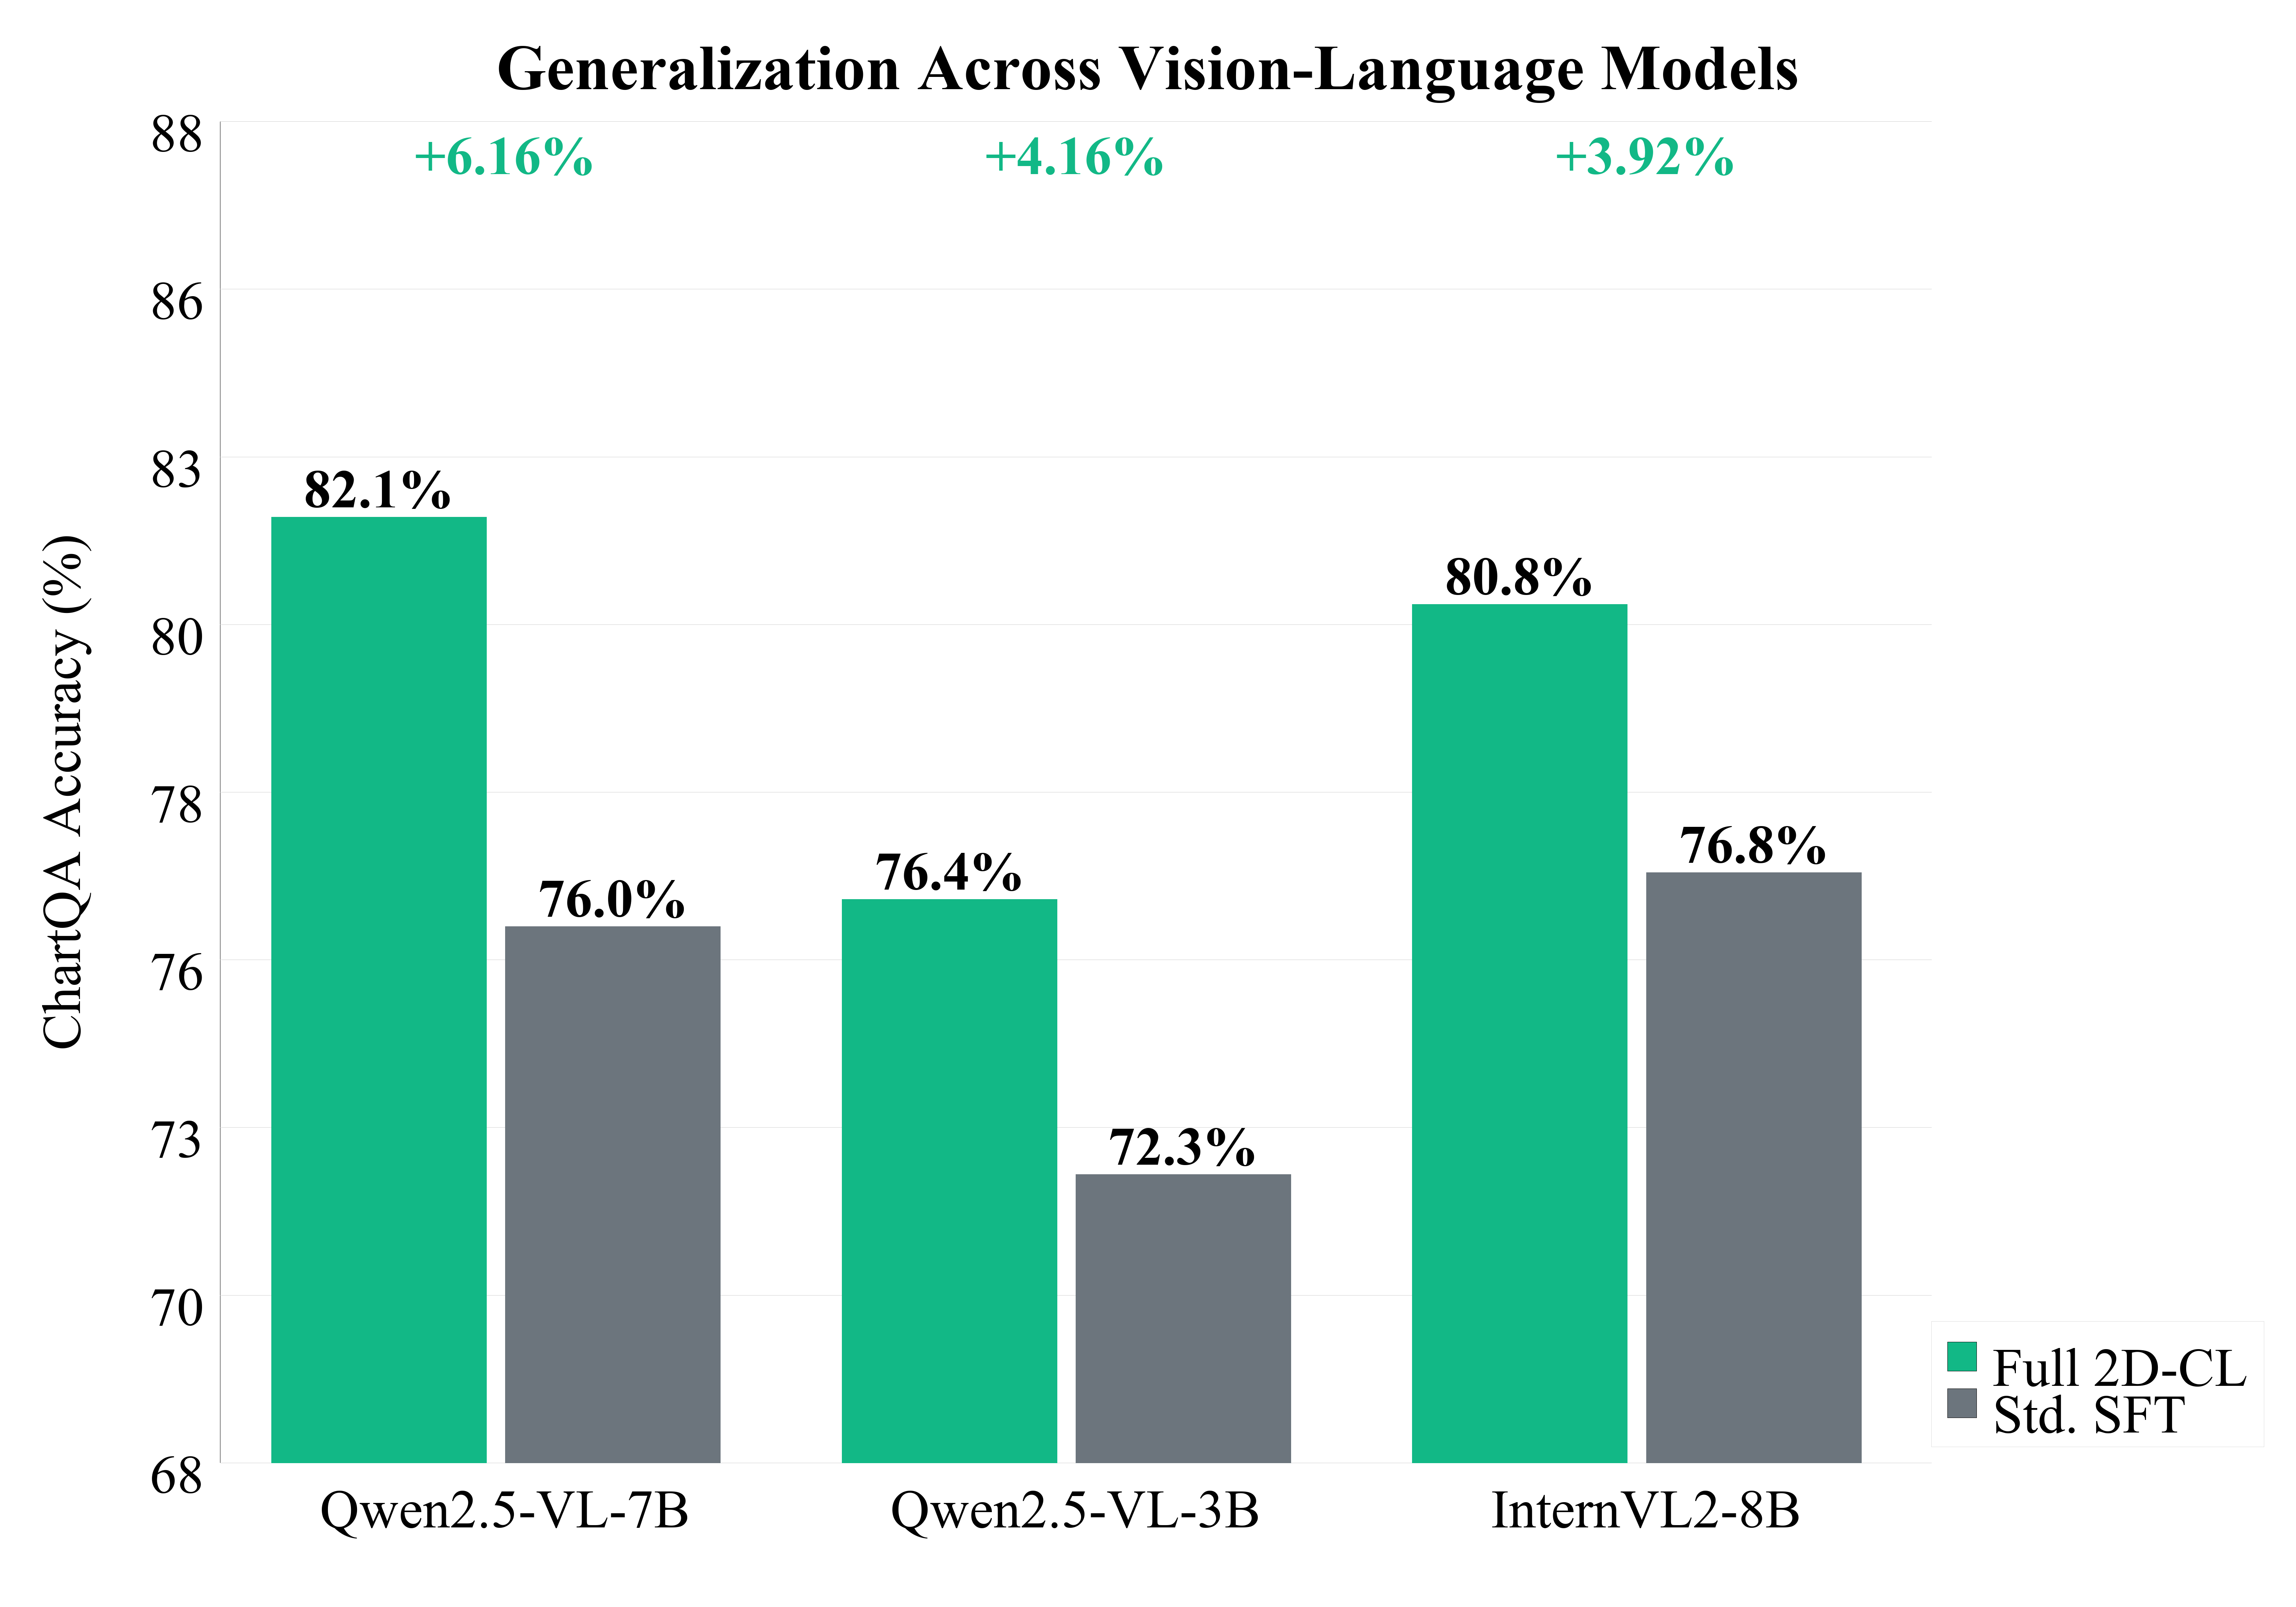
\includegraphics[width=0.32\textwidth]{figs/fig5_multi_model_comparison.png}\label{fig:exp_models}}
    \hfil
    \subfloat[Cross-dataset transfer]{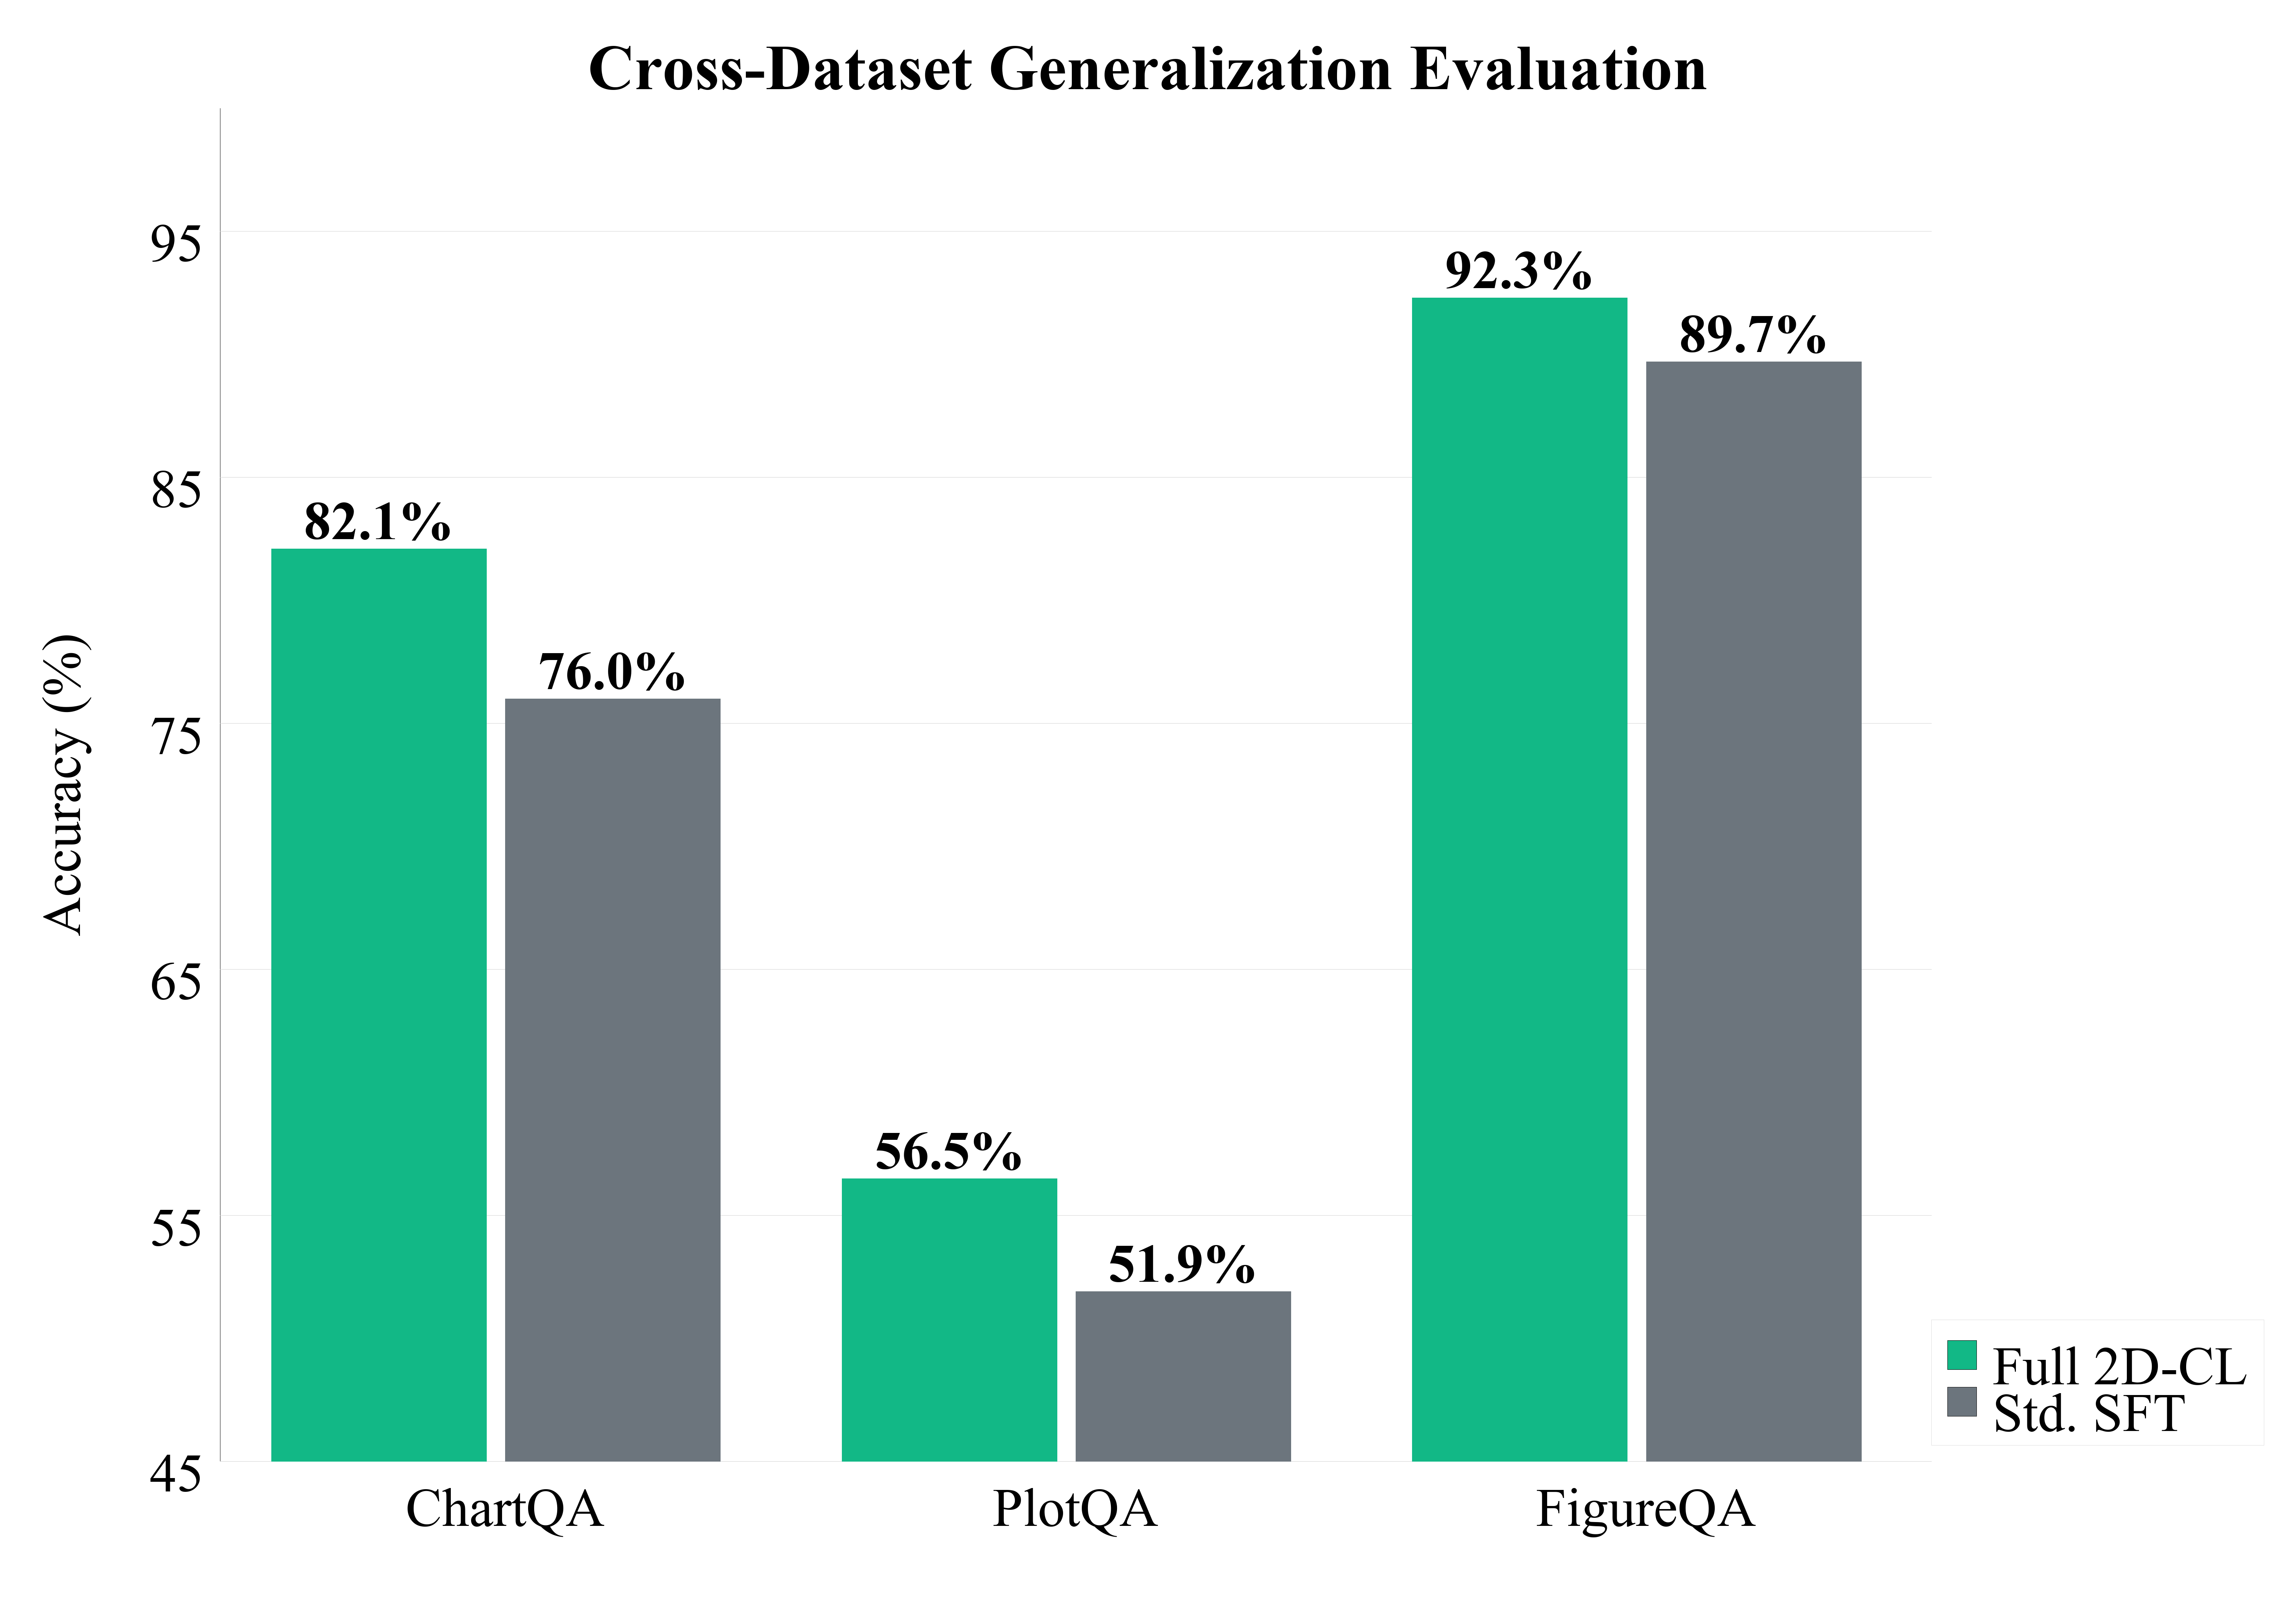
\includegraphics[width=0.32\textwidth]{figs/fig6_cross_dataset_evaluation.png}\label{fig:exp_transfer}}
    \caption{Comprehensive experimental results. (a) Each \method{} component contributes positively; adapter inheritance and task staging provide the largest gains. (b) \method{} consistently improves models across architectures and scales. (c) Strong zero-shot transfer to unseen datasets confirms generalization.}
    \label{fig:main_experiments}
\end{figure*}

\begin{table}[!t]
\centering
\small
\begin{tabular}{lccc}
\toprule
\textbf{Model} & \textbf{\method{}} & \textbf{Std. SFT} & \textbf{$\Delta$} \\
\midrule
Qwen2.5-VL-7B & 82.12 & 75.96 & +6.16 \\
Qwen2.5-VL-3B & 76.44 & 72.28 & +4.16 \\
InternVL2-8B & 80.76 & 76.84 & +3.92 \\
\bottomrule
\end{tabular}
\caption{Cross-model evaluation on ChartQA.}
\label{tab:models}
\end{table}

\begin{table}[!t]
\centering
\small
\begin{tabular}{lccc}
\toprule
\textbf{Dataset} & \textbf{\method{}} & \textbf{Std. SFT} & \textbf{$\Delta$} \\
\midrule
ChartQA & 82.12 & 75.96 & +6.16 \\
PlotQA & 56.5 & 51.9 & +4.6 \\
FigureQA & 92.3 & 89.7 & +2.6 \\
\bottomrule
\end{tabular}
\caption{Zero-shot transfer. Models trained on our synthetic data are evaluated on PlotQA and FigureQA without fine-tuning.}
\label{tab:transfer}
\end{table}

Fig.~\ref{fig:main_experiments} visualizes the three core experimental dimensions. We discuss each in turn.

\paragraph{Cross-Model Generalization.}
A natural question is whether \method{} works only for Qwen2.5-VL-7B or generalizes to other models. Table~\ref{tab:models} and Fig.~\ref{fig:exp_models} provide an answer: the curriculum helps across the board. On the smaller Qwen2.5-VL-3B, \method{} improves accuracy from 72.28\% to 76.44\% (+4.16\%). On InternVL2-8B, which uses an entirely different architecture (InternViT for vision, InternLM2 for language), the gain is +3.92\%. Larger models with more capacity appear better positioned to exploit the curriculum, though even the 3B model sees meaningful improvement.

\paragraph{Cross-Dataset Transfer.}
If \method{} merely overfits to the style of our synthetic training charts, we would expect performance to collapse on datasets with different visual characteristics. Table~\ref{tab:transfer} and Fig.~\ref{fig:exp_transfer} suggest otherwise.

PlotQA features scientific plots from research papers---a domain quite different from our business-oriented training data, with questions requiring reasoning over trends. Despite this shift, \method{} achieves 56.5\% accuracy, a 4.6\% improvement over standard LoRA SFT. FigureQA uses programmatically generated charts with binary yes/no questions, a format substantially different from our open-ended training questions. Still, \method{} reaches 92.3\% (+2.6\%).

The consistency of improvements across three datasets with distinct visual styles and question formats supports the claim that \method{} builds general chart understanding capabilities rather than dataset-specific shortcuts.

\section{Analysis}
\subsection{Stage-Specific Expertise}
One of the more revealing properties of \method{} is that each training stage produces a model with distinct strengths. Table~\ref{tab:stage_performance} breaks down performance on our five internal task types across all stages. The diagonal pattern is striking: Stage 1 excels at description (25.0 BLEU vs.\ 4.8 for the baseline), Stage 3 achieves perfect accuracy on reasoning (100\%), and Stage 5 nails code generation (100\%). What emerges is not one generalist model but a family of experts, each tuned for a specific capability.

\begin{table}[!t]
\centering
\small
\begin{tabular}{lccccc}
\toprule
& \textbf{T1} & \textbf{T2} & \textbf{T3} & \textbf{T4} & \textbf{T5} \\
& Desc. & VQA & Reas. & Vis. & Code \\
\midrule
Baseline & 4.8 & 19.2 & 84.3 & 36.9 & 14.1 \\
Stage 1 & \textbf{25.0} & 11.6 & 72.7 & 43.2 & 11.6 \\
Stage 2 & 5.2 & \textbf{24.2} & 25.8 & 46.1 & 48.0 \\
Stage 3 & 6.8 & 26.3 & \textbf{100.0} & 50.2 & 96.0 \\
Stage 4 & 8.0 & 24.7 & 81.3 & \textbf{81.3} & 48.5 \\
Stage 5 & 3.8 & 23.2 & 61.1 & 74.8 & \textbf{100.0} \\
\bottomrule
\end{tabular}
\caption{Performance on internal tasks across training stages. T1 is measured by BLEU; T2--T5 by accuracy (\%). Each stage peaks on its designated task. The internal evaluation set contains 198 samples per task; the 100\% scores on T3 and T5 reflect both this limited scale and the high format consistency between synthetic training and evaluation data.}
\label{tab:stage_performance}
\end{table}

A glance at Table~\ref{tab:stage_performance} might raise concern: by Stage 5, description BLEU has dropped to 3.8---worse than the baseline. Does the model ``forget'' how to describe charts? Not exactly. What we observe is LoRA adapter specialization rather than catastrophic forgetting in the traditional sense. Because we save separate adapters at each stage, users can select the one that matches their deployment scenario. The tradeoff between generality and specialization is explicit and controllable.

The 100\% scores on T3 and T5 warrant comment. These reflect the internal evaluation set (198 samples per task), where format consistency between training and test data is high. On the external ChartQA benchmark (2,500 questions with diverse visual styles and question formats), the best stage achieves 82.12\%---a more nuanced picture. The internal metrics are best interpreted as indicators of \emph{relative} stage specialization rather than absolute capability claims.

\subsection{The Role of Code-as-Reasoning Supervision}
\begin{figure}[!t]
    \centering
    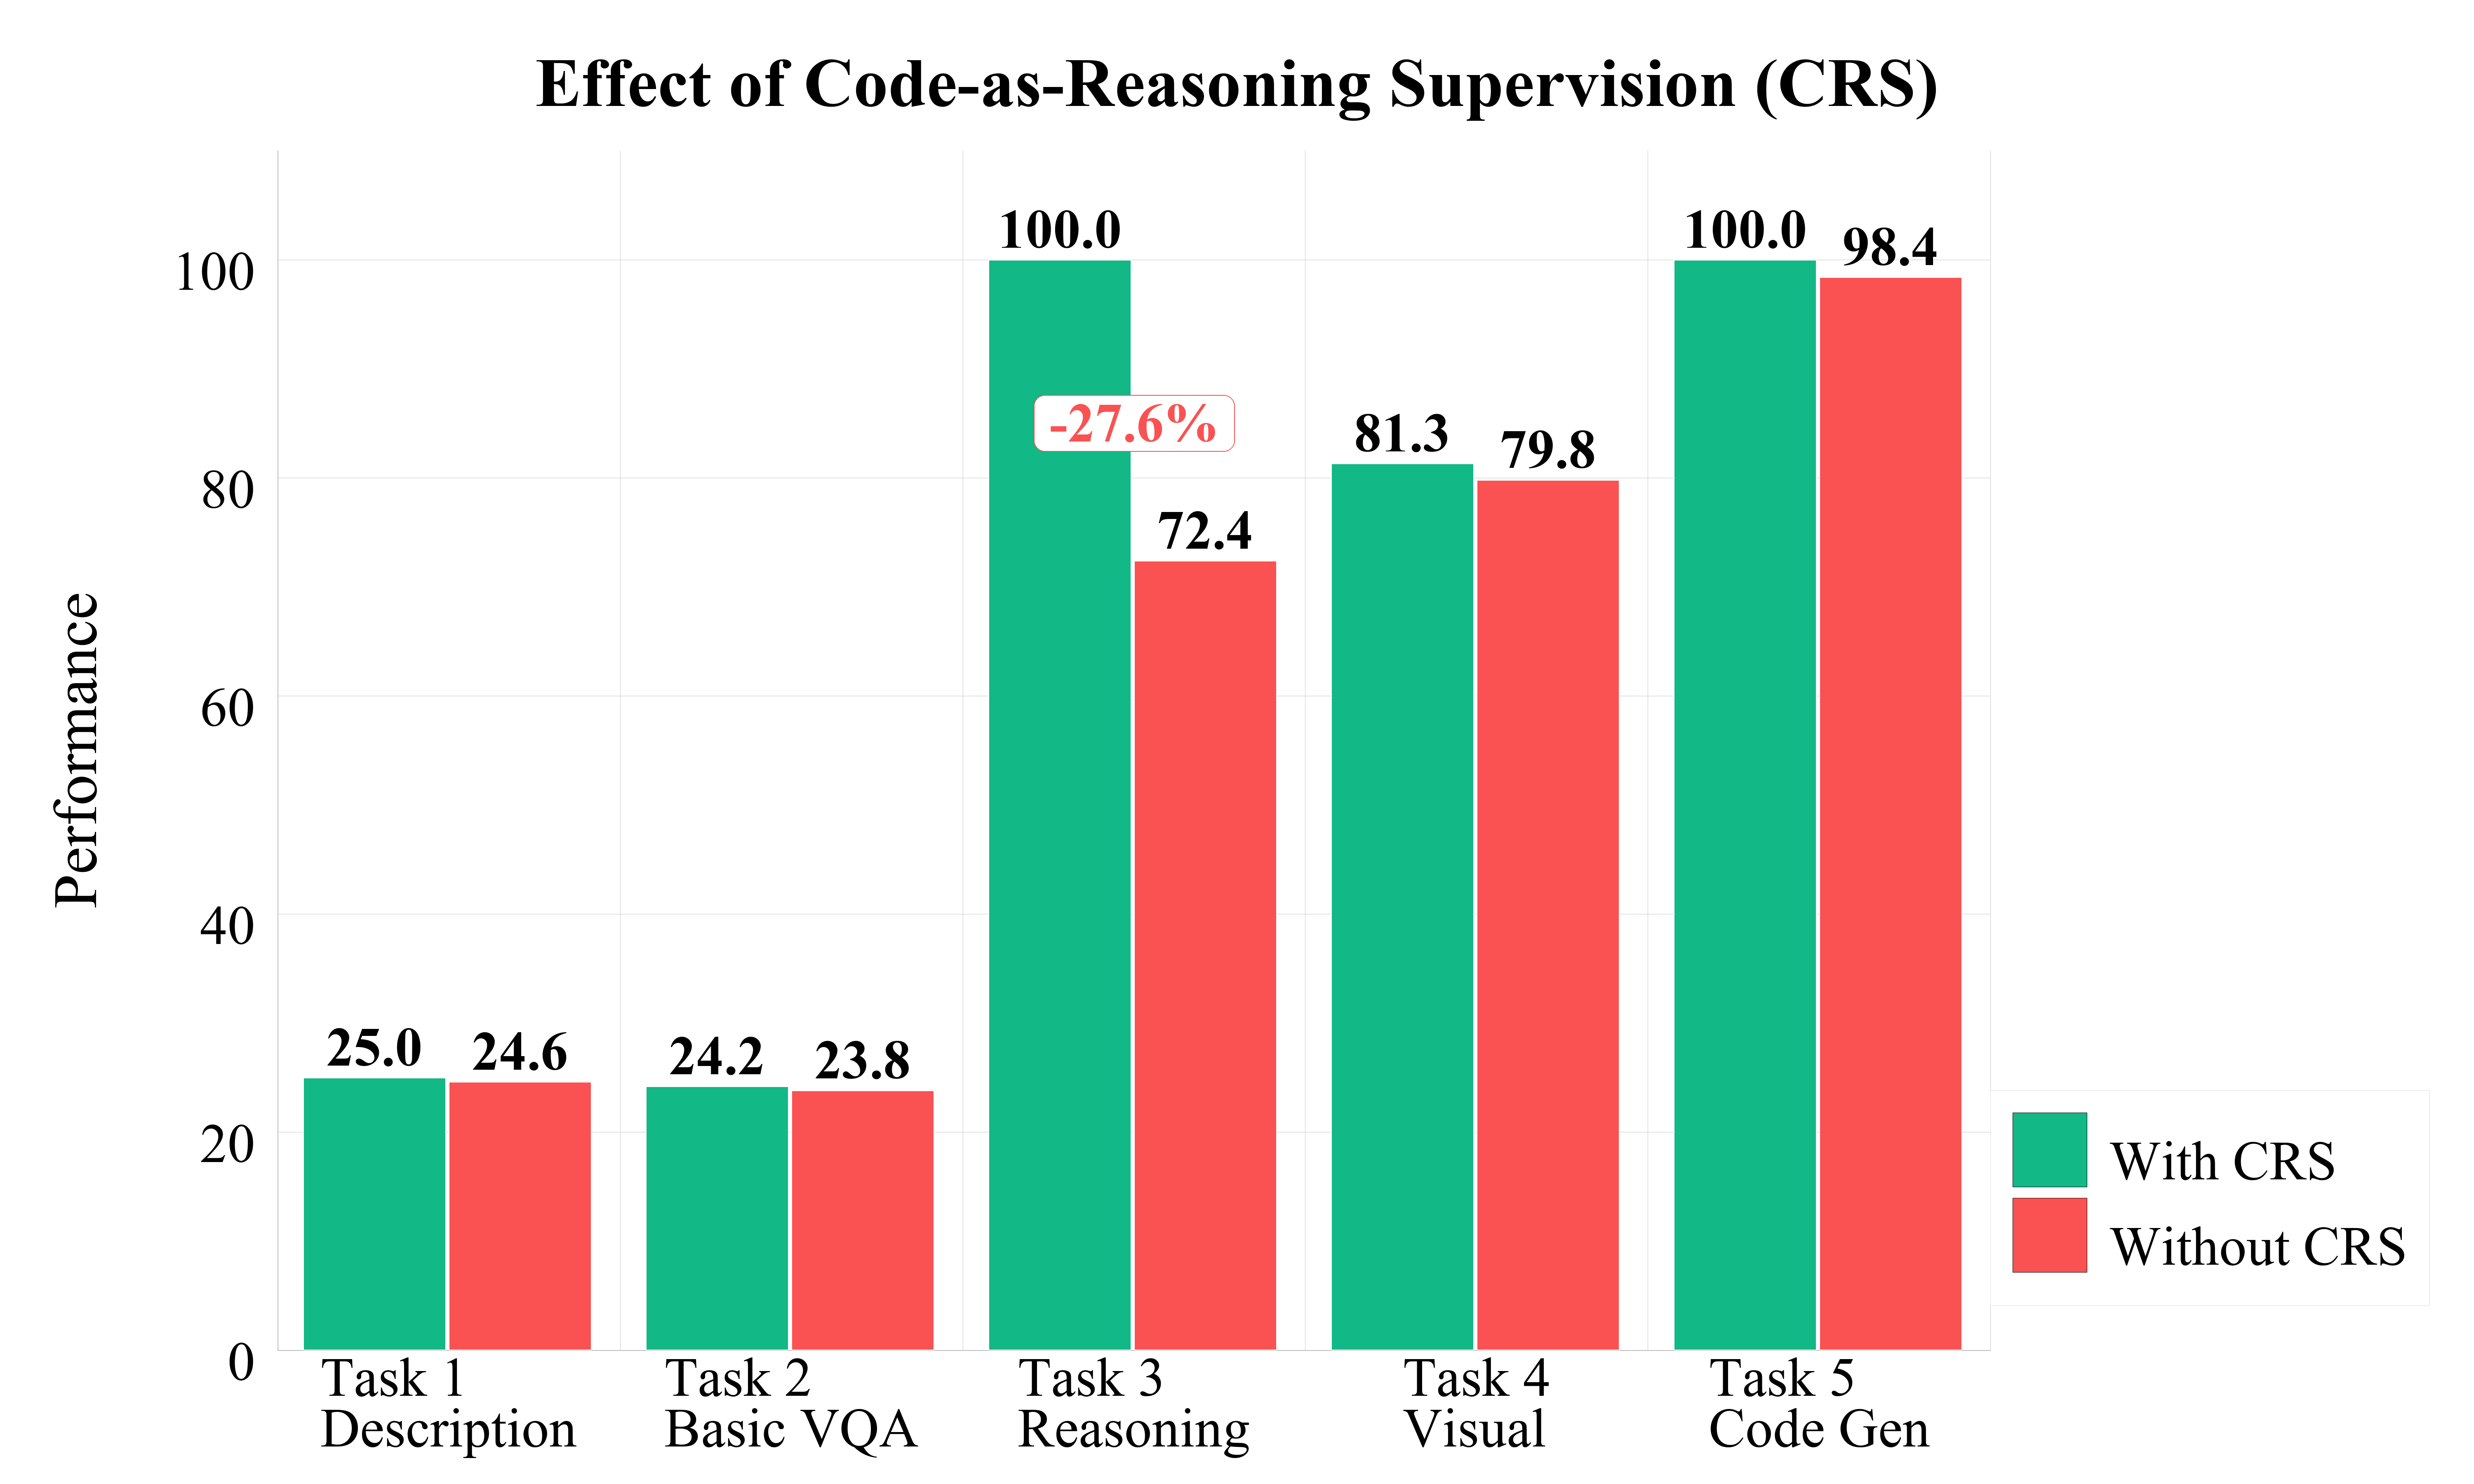
\includegraphics[width=\columnwidth]{figs/fig10_crs_effect.png}
    \caption{Impact of \crs{} across task types. Removing code-based reasoning supervision from Stage 3 causes accuracy on reasoning tasks to drop from 100\% to 72.4\%, while other tasks are less affected.}
    \label{fig:crs_effect}
\end{figure}

Fig.~\ref{fig:crs_effect} isolates the effect of \crs{} at a per-task level. The asymmetry is informative: removing \crs{} devastates Task 3 (Reasoning: 100\% $\rightarrow$ 72.4\%) but barely affects other tasks. This confirms that \crs{} targets a specific capability gap rather than providing a general training bonus. The baseline model already possesses substantial reasoning ability (84.3\% on Task 3 without any fine-tuning), but direct QA-style training in Stage 2 actually \emph{degrades} this capability to 25.8\%---likely because Stage 2's short-answer format conflicts with the verbose reasoning the model needs to perform. \crs{} not only recovers but perfects reasoning by providing the right kind of supervision: structured, step-by-step, and verifiable.

\subsection{Why Adapter Inheritance Matters Most}
The ablation study singled out adapter inheritance as the largest contributor (+4.80\%), which warrants deeper examination. Without inheritance, each stage initializes from the pretrained VLM and trains in isolation. The five stages effectively become five independent fine-tuning runs that happen to use different data.

Why does this hurt so much? Consider the pathway from Stage 1 to Stage 3. Stage 1 teaches the model to attend to visual details---axis labels, legend entries, data point positions---through the description task. Stage 2 converts this visual attention into value extraction for QA. Stage 3 then builds reasoning on top of reliable extraction. Without inheritance, Stage 3 must simultaneously learn visual grounding \emph{and} reasoning from scratch, using only 1,775 reasoning-focused samples. With inheritance, it can focus entirely on reasoning because the perceptual foundation is already in place.

This finding aligns with a broader principle in curriculum learning: the curriculum is only effective when knowledge flows cumulatively from earlier to later stages. An ordered sequence of tasks without a mechanism for retention is just a series of unrelated training runs.

\subsection{Qualitative Examples}
To ground the quantitative results, we present representative cases from our ChartQA evaluation.

\paragraph{How \crs{} Structures Reasoning.}
The following example illustrates the step-by-step reasoning pattern that Stage 3 learns through \crs{}. Given a chart and the question ``\textit{What percentage of the total does Bus represent?}'', the model produces:
\begin{small}
\begin{quote}
\textit{Step 1:} Read the Bus value from the chart (84). \\
\textit{Step 2:} Sum all values to obtain the total (84+40+28+53+42+25=272). \\
\textit{Step 3:} Divide Bus by total to get the proportion. \\
\textit{Step 4:} Multiply by 100: $84/272 \approx$ 30.88\%.
\end{quote}
\end{small}
Each step is grounded in a concrete operation---value extraction, summation, division---leaving little room for shortcuts. This structured decomposition is what \crs{} teaches during training; at inference on ChartQA, the model uses the Stage 2 adapter to produce direct answers, but the internalized reasoning patterns carry over through adapter inheritance.

\paragraph{Format Learning.}
A recurring pattern in our evaluation is that the baseline model often \emph{knows} the answer but buries it in a verbose response that fails exact-match evaluation. For instance, when asked ``\textit{Is the sum of Charismatic and Well-qualified to be president more than A strong leader?}'', the baseline extracts the correct values (39\%+26\%=65\% $>$ 55\%) but generates a multi-sentence explanation that gets truncated before stating ``Yes.'' After Stage 2 training, the model learns to respond concisely: ``Yes.'' This is not a reasoning improvement but a \emph{format} improvement---the curriculum teaches the model to match the expected output format, which is a prerequisite for benchmark performance.

\paragraph{Persistent Errors.}
Not all errors are resolved by the curriculum. When asked ``\textit{How many food items are shown in the bar graph?}'' (gold: 14), the model answers ``15'' across all stages, including the baseline. This counting error persists because it stems from low-level visual perception---miscounting closely packed bars in a dense chart---rather than from reasoning deficits. The 2D curriculum improves reasoning and format but does not fundamentally alter the base model's visual encoder, which remains frozen during LoRA training.

\subsection{Training Efficiency}
The curriculum proceeds smoothly from a computational standpoint. Training loss falls from 0.667 at the end of Stage 1 to 0.110 by Stage 5---an 83.4\% reduction---with no abrupt spikes or instabilities along the way. Total training time for the full five-stage pipeline is about 21 hours on a single GPU, and each adapter adds only 77MB of storage. This makes it practical to maintain and deploy a suite of specialized models without prohibitive overhead.

\section{Conclusion}
We have presented \fullmethod{}, a framework that organizes chart understanding training along two axes: task complexity and sample difficulty. The horizontal curriculum decomposes the problem into five stages---description, basic QA, reasoning, visual analysis, code generation---while the vertical curriculum orders samples within each stage from easy to hard. Two technical innovations support this structure: Code-as-Reasoning Supervision, which provides explicit step-by-step reasoning annotations via executable code, and Difficulty-Aware Curriculum Data Selection, which uses an LLM to score sample difficulty.

On ChartQA, this approach yields 82.12\% accuracy with a 7B model trained on only 12K synthetic samples---a 6.16\% improvement over standard LoRA fine-tuning on the same data, demonstrating that curriculum structure provides substantial gains beyond what unstructured training can achieve. Ablation studies isolate the contribution of each component, with adapter inheritance and task staging providing the largest gains. The method generalizes across model architectures and transfers to unseen benchmarks, suggesting that the learned capabilities are fundamental rather than dataset-specific.

Our results point to a broader lesson: for complex visual understanding tasks that involve multiple interrelated skills, the structure of training can matter as much as data scale or model size. By decomposing chart understanding into a principled sequence of capabilities and providing the right form of supervision at each stage, we achieve competitive performance with modest resources. The \crs{} technique, in particular, may find applications beyond chart understanding wherever multi-step computation over visual inputs is needed.

\section*{Limitations}
Several limitations of this work deserve mention.

\paragraph{Scale of Training Data.}
Our experiments use roughly 12K synthetic samples---a deliberately modest amount intended to test whether curriculum structure can substitute for data volume. Whether scaling up the data would yield further gains, and how the curriculum's relative benefit might change at larger scale, remains an open question.

\paragraph{Chart Type Coverage.}
The synthetic data generation covers five chart types: bar, line, pie, scatter, and area charts. More specialized visualizations---geographical maps, network diagrams, Sankey charts, 3D plots---fall outside the current scope. Extending the framework to these would require additional data generation and possibly task definitions tailored to their unique characteristics.

\paragraph{Language.}
All experiments are conducted in English. Charts in other languages, or multilingual settings where the chart text is in one language and the question in another, are not addressed. Adapting \method{} to multilingual chart understanding would require cross-lingual training data and evaluation.

\paragraph{Adapter Management.}
While LoRA adapters are lightweight (77MB each), maintaining five separate adapters per model introduces deployment complexity. In production, one must either choose a single adapter or implement routing logic to select the appropriate adapter based on query characteristics. A single unified model would be more convenient, though it might sacrifice the specialization benefits observed here.

\paragraph{Statistical Significance.}
All reported results are from single training runs with fixed random seeds. While LoRA fine-tuning typically exhibits low variance across runs---prior work on comparable setups reports standard deviations of $\pm$0.3--0.5\% on benchmarks of similar scale~\cite{hu2022lora}---we acknowledge that multi-run evaluation with confidence intervals would strengthen our claims, particularly for the smaller improvements such as the 1.28\% contribution of difficulty ordering.

\paragraph{Evaluation Breadth.}
Our primary evaluation centers on ChartQA, the most established chart QA benchmark. While we include zero-shot transfer results on PlotQA and FigureQA, a more comprehensive evaluation on recently proposed benchmarks such as ChartBench and OpenCQA would further validate generalizability. We prioritize depth of analysis on a single well-understood benchmark---including ablation studies, cross-model experiments, and stage-specific evaluation---over breadth across multiple benchmarks, but recognize that broader evaluation remains valuable future work.

\appendices
\section{Training Details}
\paragraph{Dataset Composition.}
Fig.~\ref{fig:dataset_dist} visualizes the composition of our synthetic training data. The chart type distribution is roughly balanced, with bar charts (27.5\%) and line charts (25.7\%) slightly overrepresented compared to area charts (9.8\%). Across ten scenario categories, business (380 charts) and science (320 charts) are most prevalent, reflecting domains where charts commonly appear. Difficulty levels skew toward lower values by design---consistent with the curriculum philosophy of providing more easy examples---though all five levels are represented.

\begin{figure}[!t]
    \centering
    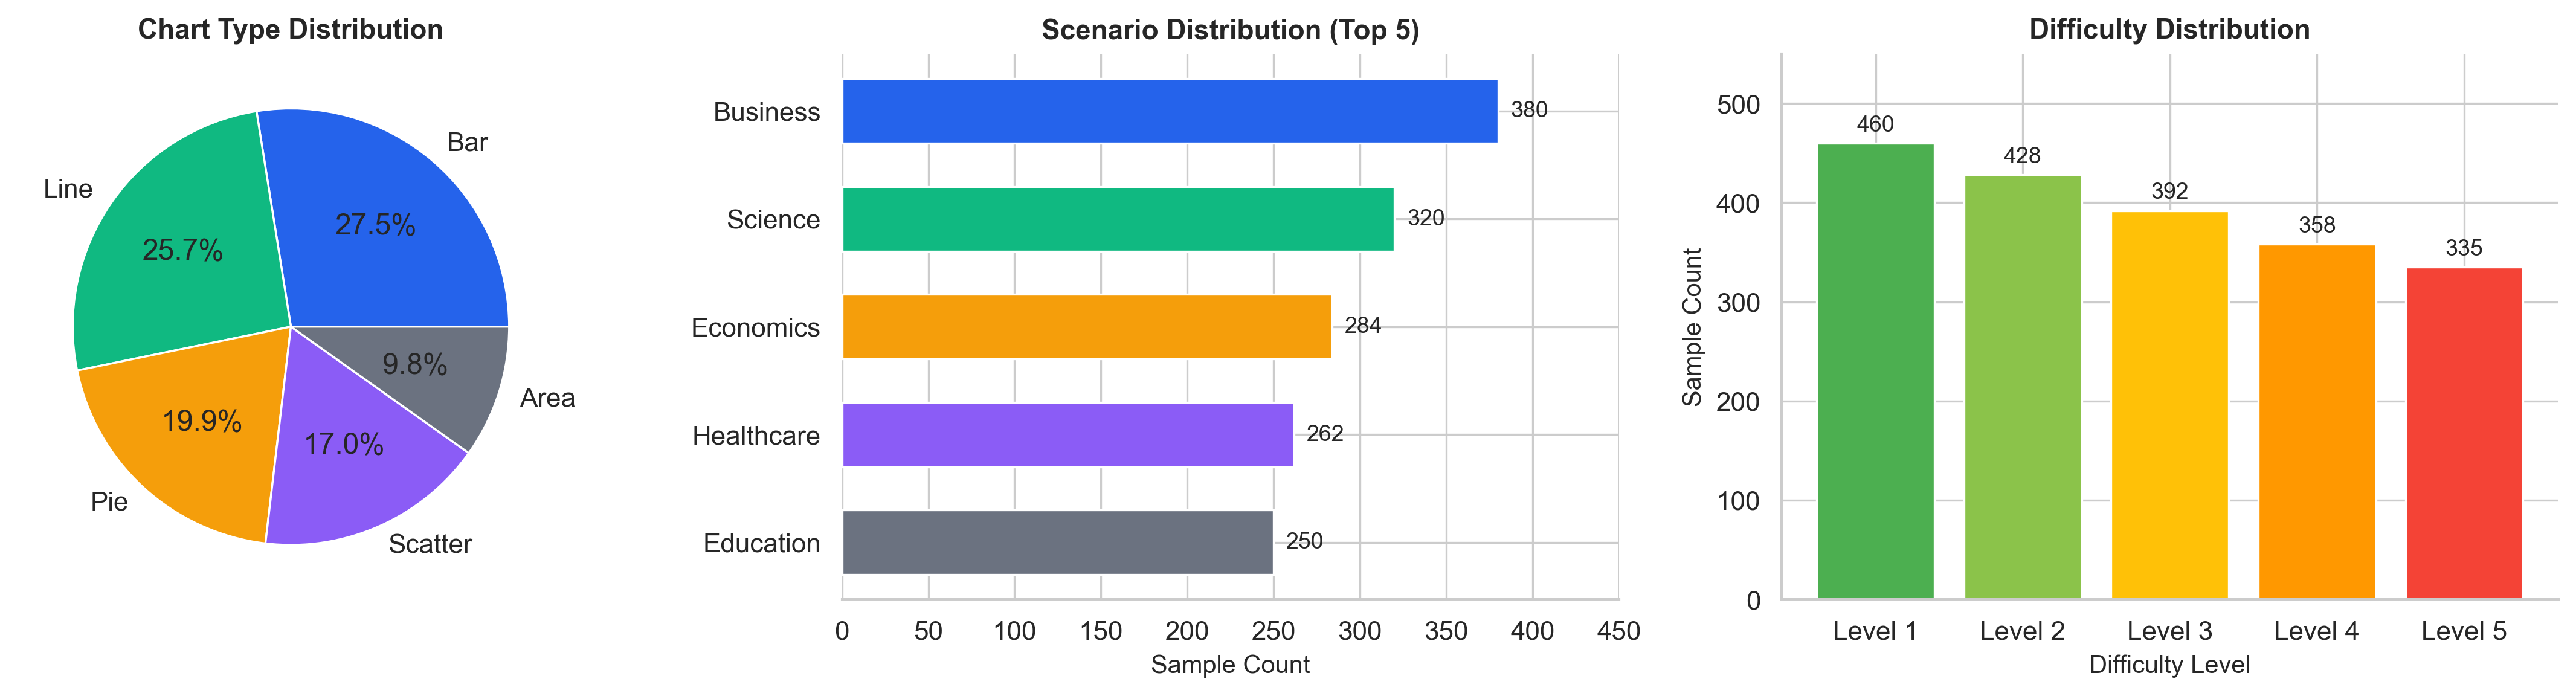
\includegraphics[width=\columnwidth]{figs/fig11_dataset_distribution.png}
    \caption{Distribution of synthetic training data. (a) Chart types. (b) Scenario categories. (c) Difficulty levels, showing more samples at lower difficulty as intended by the curriculum.}
    \label{fig:dataset_dist}
\end{figure}

\paragraph{Hyperparameters.}
Table~\ref{tab:hyperparams} lists the complete hyperparameter settings for each training stage. Learning rates decrease across stages on the rationale that earlier stages establish coarse-grained capabilities while later stages refine them. Stage 5 uses a longer maximum sequence length (4096 tokens) to accommodate code generation outputs.

\begin{table}[!t]
\centering
\small
\begin{tabular}{lccccc}
\toprule
& \textbf{S1} & \textbf{S2} & \textbf{S3} & \textbf{S4} & \textbf{S5} \\
\midrule
Learning Rate & 1e-4 & 5e-5 & 3e-5 & 3e-5 & 2e-5 \\
Epochs & 10 & 10 & 10 & 10 & 10 \\
Batch Size & 16 & 16 & 16 & 16 & 16 \\
Max Length & 2048 & 2048 & 2048 & 2048 & 4096 \\
Warmup Ratio & 0.05 & 0.05 & 0.05 & 0.05 & 0.05 \\
Weight Decay & 0.01 & 0.01 & 0.01 & 0.01 & 0.01 \\
LoRA Rank & 8 & 8 & 8 & 8 & 8 \\
LoRA Alpha & 16 & 16 & 16 & 16 & 16 \\
LoRA Dropout & 0.1 & 0.1 & 0.1 & 0.1 & 0.1 \\
\bottomrule
\end{tabular}
\caption{Hyperparameters for each training stage.}
\label{tab:hyperparams}
\end{table}

\paragraph{Training Dynamics.}
Table~\ref{tab:training_dynamics} summarizes the convergence behavior of each stage. All stages exhibit stable convergence without erratic fluctuations, and the final loss forms a monotonically decreasing sequence from 0.667 (Stage~1) to 0.110 (Stage~5)---an overall reduction of 83.4\%. This pattern suggests that the model progressively internalizes the curriculum, with each stage starting from a better initialization (via adapter inheritance) and converging to a lower optimum.

\begin{table}[!t]
\centering
\small
\begin{tabular}{lccccc}
\toprule
& \textbf{S1} & \textbf{S2} & \textbf{S3} & \textbf{S4} & \textbf{S5} \\
\midrule
\# Samples & 1,775 & 1,775 & 1,775 & 5,327 & 1,775 \\
Initial Loss & 2.34 & 1.18 & 0.86 & 0.58 & 0.42 \\
Final Loss & 0.667 & 0.376 & 0.274 & 0.177 & 0.110 \\
Reduction (\%) & 71.5 & 68.1 & 68.1 & 69.5 & 73.8 \\
Epochs to 90\% & 3 & 2 & 2 & 4 & 2 \\
Wall-clock (h) & 3.6 & 2.7 & 2.5 & 9.6 & 2.5 \\
\bottomrule
\end{tabular}
\caption{Training dynamics across stages. ``Epochs to 90\%'' indicates how many epochs are needed to reach 90\% of the final performance. Stage 4 takes the longest due to its $3\times$ larger sample count.}
\label{tab:training_dynamics}
\end{table}

Two observations stand out. The first is convergence speed: most stages reach 90\% of their final performance within the first 2 epochs, indicating that the curriculum ordering provides effective initialization. Stage 4 (Visual Analysis) is the exception, requiring 4 epochs, likely because its three subtasks introduce more diverse gradients. The second observation concerns total wall-clock time: the full five-stage pipeline completes in roughly 20.9 hours on a single NVIDIA RTX 5090 GPU, with Stage 4 accounting for nearly half of this budget due to its $3\times$ larger sample count.

\section{Additional Results}
\paragraph{Component Contributions.}
Table~\ref{tab:component_detail} quantifies the contribution of each \method{} component measured as the accuracy drop on ChartQA when that component is removed from the full system. Adapter inheritance contributes the most (+4.80\%), followed by task staging (+3.48\%), \crs{} (+2.64\%), and difficulty ordering (+1.28\%). The four contributions sum to 12.20\%, which exceeds the 6.16\% total improvement over the random baseline---evidence that the components interact positively and that disrupting any one of them has cascading effects on the others.

\begin{table}[!t]
\centering
\small
\begin{tabular}{lcc}
\toprule
\textbf{Component Removed} & \textbf{Acc. (\%)} & \textbf{$\Delta$ vs.\ Full} \\
\midrule
\textit{Full \method{}} & \textit{82.12} & --- \\
\midrule
w/o Adapter Inheritance & 77.32 & $-4.80$ \\
w/o Task Staging & 78.64 & $-3.48$ \\
w/o CRS & 79.48 & $-2.64$ \\
w/o Difficulty Ordering & 80.84 & $-1.28$ \\
\midrule
Random Baseline & 75.96 & $-6.16$ \\
\bottomrule
\end{tabular}
\caption{Individual contribution of each component to ChartQA accuracy, measured as the drop when the component is removed.}
\label{tab:component_detail}
\end{table}

\paragraph{Multi-Task Performance Profile.}
Table~\ref{tab:task_profile} compares the full \method{} and random baseline across all five internal task types. The curriculum yields consistent improvements, but the gains are concentrated on the reasoning and code generation tasks---precisely those that demand multi-step thinking. On simpler tasks (description, basic VQA), the gap narrows, suggesting that the pretrained model already handles these reasonably well and the curriculum's added value lies primarily in structured reasoning capabilities.

\begin{table}[!t]
\centering
\small
\begin{tabular}{lcc}
\toprule
\textbf{Task Type} & \textbf{\method{}} & \textbf{Random} \\
\midrule
T1: Description (BLEU) & 25.0 & 12.8 \\
T2: Basic VQA (Acc.) & 24.2 & 18.2 \\
T3: Reasoning (Acc.) & 100.0 & 58.4 \\
T4: Visual Analysis (Acc.) & 81.3 & 54.6 \\
T5: Code Generation (Acc.) & 100.0 & 62.4 \\
\bottomrule
\end{tabular}
\caption{Performance comparison across five task types. The curriculum's largest gains appear on reasoning-heavy tasks (T3, T5).}
\label{tab:task_profile}
\end{table}

\paragraph{Training Efficiency.}
Table~\ref{tab:efficiency} reports training time and convergence speed by stage. Stage 4 consumes the most wall-clock time (9.6 hours) because it contains roughly $3\times$ more samples than other stages. Despite this, all stages converge efficiently: the average number of epochs to reach 90\% of final performance is 2.6, indicating that the curriculum ordering and adapter inheritance together provide effective initialization. The total storage overhead of the LoRA adapters is modest---approximately 77MB per adapter, or 385MB for the full five-stage set.

\begin{table}[!t]
\centering
\small
\begin{tabular}{lccccc}
\toprule
& \textbf{S1} & \textbf{S2} & \textbf{S3} & \textbf{S4} & \textbf{S5} \\
\midrule
Time (hours) & 3.6 & 2.7 & 2.5 & 9.6 & 2.5 \\
Epochs to 90\% & 3 & 2 & 2 & 4 & 2 \\
Adapter Size (MB) & 77 & 77 & 77 & 77 & 77 \\
\bottomrule
\end{tabular}
\caption{Training efficiency metrics per stage. Total training time is 20.9 hours on a single NVIDIA RTX 5090 GPU.}
\label{tab:efficiency}
\end{table}

\bibliographystyle{IEEEtran}
\bibliography{references}

\end{document}
